% !TEX root = ../BScWIMEngl.tex  

\chapter{Markov Decision Processes}
\section{Introduction}
I will try to convey intuition for Markov Decision Processes in this Introduction. Readers familiar with the subject can skip directly to the formal model formulation. 

A Markov Decision Process appears to be quite similar to a Markov Process at first glance. Where a Markov Process is a stochastic process, i.e. a sequence of random variables \((X_t,t\in\N_0)\), which is memoryless (Markov). This means knowledge of the current state, makes knowledge about past states useless for predicting future states.

Markov Decision Processes (MDPs) introduce actions \((A_t,t\in\N_0)\) and rewards \((R_t,t\in\N)\) to this model. Where the transition to the next state \(X_{t+1}\) given a state \(X_{t}\) and action \(A_{t}\) is Markov (memoryless), just like in Markov Processes.
\[
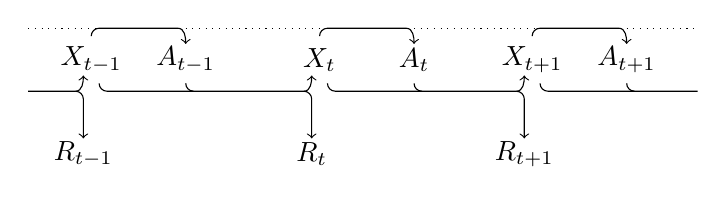
\begin{tikzpicture}
    \draw[dotted] (-3.7,0.4) -- (-2.8,0.4);

    \draw[->] (-3.7, -0.4) %%% transition stub beginning
    to [out=0,in=180] (-3.1, -0.4)
    to [out=0,in=270] (-3, -0.2);

    \draw[->] (-3.1, -0.4) %%% to R_{t-1}
    to [out=0,in=90] (-3,-0.5)
    to [out=270, in=90] (-3,-1);

    \draw (-3,-1.2) node {\(R_{t-1}\)};
    \draw (-2.9,0) node {\(X_{t-1}\)};

    \draw[->] (-2.9,0.3) %%% X_{t-1} to A_{t-1}
    to [out=90,in=180] (-2.8, 0.4) 
    to [out=0,in=180] (-1.8,0.4)
    to [out=0,in=90] (-1.7,0.2);

    \draw[dotted] (-1.7,0.4) -- (0.1,0.4);

    \draw (-1.7,0) node {\(A_{t-1}\)};

    \draw (-1.7, -0.3) %%% join transition 
    to [out=270,in=180] (-1.6,-0.4);

    \draw[->] (-2.8, -0.3) %%% X_{t-1} to X_t transition
    to [out=270,in=180] (-2.7, -0.4) 
    to [out=0,in=180] (-0.2, -0.4)
    to [out=0,in=270] (-0.1, -0.2);

    \draw[->] (-0.2, -0.4) %%% to R_t
    to [out=0,in=90] (-0.1,-0.5)
    to [out=270, in=90] (-0.1,-1);

    \draw (-0.1,-1.2) node {\(R_t\)};
    \draw (0,0) node {\(X_t\)};
    
    \draw[->] (0,0.3)  %%% X_t to A_t
    to [out=90,in=180] (0.1, 0.4) 
    to [out=0,in=180] (1.1,0.4)
    to [out=0,in=90] (1.2,0.2); 

    \draw[dotted] (1.2,0.4) -- (2.8,0.4);
 
    \draw (1.2,0) node {\(A_t\)};

    \draw (1.2, -0.3) %%% join transition
    to [out=270,in=180] (1.3,-0.4);

    \draw[->] (0.1, -0.3) %%% X_t to X_{t+1} transition
    to [out=270,in=180] (0.2, -0.4) 
    to [out=0,in=180] (2.5, -0.4)
    to [out=0,in=270] (2.6, -0.2);

    \draw[->] (2.5, -0.4) %%% to R_{t+1}
    to [out=0,in=90] (2.6,-0.5)
    to [out=270, in=90] (2.6,-1);

    \draw (2.6,-1.2) node {\(R_{t+1}\)};
    \draw (2.7,0) node {\(X_{t+1}\)};

    \draw[->] (2.7,0.3)  %%% X_{t+1} to A_{t+1}
    to [out=90,in=180] (2.8, 0.4) 
    to [out=0,in=180] (3.8,0.4)
    to [out=0,in=90] (3.9,0.2); 

    \draw[dotted] (3.9,0.4) -- (4.8,0.4);

    \draw (3.9,0) node {\(A_{t+1}\)};

    \draw (3.9, -0.3) %%% join transition stub
    to [out=270,in=180] (4,-0.4);

    \draw (2.8, -0.3) %%% X_{t+1} transition stub end
    to [out=270,in=180] (2.9, -0.4) 
    to [out=0,in=180] (4.8, -0.4);
\end{tikzpicture}
\]
But this apparent similarity can be misleading. While Markov Processes are defined as a stochastic process (i.e. a sequence of states) with properties as described above, MDPs cannot be defined like that. The reason for this is, that the next state \(X_{t+1}\) depends on the current state and action \(A_{t}\), which means that the sequence of states cannot be defined without the sequence of actions. But defining the sequence of actions requires an action selection rule, a behaviour, a decision. So defining MDPs as a stochastic process, would result in every behaviour resulting in a different MDP. But since MDPs want to model decisions, this does not make much sense. Talking about optimal behaviours in a framework which can only be defined for a set behaviour, is nonsensical. What is needed is a model framework which is invariant to different behaviours. Therefore MDPs are not defined as a stochastic process, but rather as a rulebook on how to create a stochastic process given a behaviour. 

The questions we ask the model are also different.  MDPs are more interested into evaluating different behaviours and finding optimal ones, while Markov Processes try to describe an existing phenomenon. Though we will find, that -- given a behaviour which is memoryless as well (without the dotted lines in the diagram) -- the resulting stochastic process \((X_t,A_t,R_{t+1},t\in\N_0)\) is a Markov Process, so the theory of Markov Processes could in principle be applied. But this will not be our focus. 

Just like with Markov chains, the memorylessness could be circumvented by including the history in the current state, massively increasing the state space in the process. However it is questionable whether this would yield any interesting results, as then no state is visited twice. So it is of no use to an actor to learn the value of an action in a certain state without further assumptions.

While the theory of MDPs found an extremely broad application as the backbone for reinforcement algorithms, and by proxy robotics, more classical applications include \parencite{whiteRealApplicationsMarkov1985}:
\begin{enumerate}
	\item Resource Management: The state is the resource level
	\begin{itemize}
		\item Inventory Management: The resource is the inventory, the possible action is to order resupply, influencing the inventory (state) together with the stochastic demand, and the reward is the profit. The essential trade-off is the cost of storage versus lost sales from a stock-out.
		\item Fishing: The resource is the amount of fish, the action is the amount fished, the reward is directly proportional to the amount fished, and the repopulation is the random element.
		\item Pumped storage Hydro-power: The state is the amount of water in the higher reservoir and the electricity price, the action is to use water to generate electricity or wait for higher prices.
		\item Beds in a hospital: How many empty beds are needed for emergencies?
	\end{itemize}
	\item Stock trading: The state is the price level and stock and liquidity owned.
	\item Maintenance: When does a car/road become too expensive to repair?
	\item Evacuation in response to flood forecasts
\end{enumerate}
Lastly, to ease ourselves into the abstract definition of MDPs, let us do one example in more depth. Since examples in reinforcement learning, which make use of stochasticity, quickly become overly complex, we will stay with a classical example. Examples for reinforcement learning will naturally come up in the second chapter. 
\begin{example}[Inventory Management]\label{example: inventory mgmt} We will look at a retail store with just one good for simplicity. Let
	\begin{description}[noitemsep]
		\item[\(\cX\coloneqq\N\)] be the set of possible quantities of goods in stock,
		\item[\(\cA\coloneqq\N\)] be the set of possible orders for resupply.
	\end{description}
	We will now introduce the mechanics of actions and rewards without stochastic behaviour and then change that later.

	Let us assume that the ordered goods \(a_t\in\cA\) arrive in the morning the next day. The goods sold are the demand \(d_t\), if the current stock \(x_t\in\cX\) can meet the demand. So the amount sold is actually \(d_t\wedge x_t = \min\{d,x_t\}\). Assume orders are paid for in advance and bought at price \(1\), while the goods are sold at price \(p\). The cost of storage is \(q\) per item and day. Then the profit at the end of day \(t\) is
	\[
		r_{t+1}= p (d_t\wedge x_t)-a_t-q(x_t - d_t\wedge x_t).
	\]
	And the stock level on the next day will be
	\[
		x_{t+1}=x_t - d_t\wedge x_t + a_t.
	\]
	Defining the \emph{state transition function}
	\begin{align*}
		f(x,a,d)\coloneqq \left(x-d\wedge x + a,\; p(d\wedge x) - a - q(x - d\wedge x)\right),
	\end{align*}
	allows us to express the day to day transition as
	\[
		f(x_t,a_t,d_t)=(x_{t+1}, r_{t+1}).
	\]
	Now assume that the demand is a random variable \(D_t\) which are independent and identically distributed (iid) for all \(t\). This makes all the other objects (except for the actions) necessarily random variables too. Then distribution of \((X_{t+1},R_{t+1})\) conditional on \(X_t=x, A_t=a\) is defined to be the \emph{transition probability kernel} \(\cP\) with
	\begin{align*}
		\cP(\cdot \mid x, a)\coloneqq\Pr_{f(x,a,D_t)}\xeq{\text{iid}} \Pr_{f(x,a,D_0)}.
	\end{align*}
	Note that knowledge of the transition kernel \(\cP\) is equivalent to knowledge of the transition function \(f\) and the distribution of the demand. Transition kernels reduce the clutter caused by exogenous random variables, which are different from application to application and are unknown until the next state is realized, at which point their knowledge is useless. We will therefore define this MDP to be \(\cM=(\cX,\cA,\cP)\).

	A stationary behaviour in this example would be a probability distribution over the possible orders, given the current state, i.e.
	\begin{align*}
		\pi(\cdot \mid x) \text{ is a probability distribution over }\cA.
	\end{align*}
	Actions are then selected by picking a random variable from this distribution,
	\[
		A_t \sim \pi(\cdot \mid X_t).
	\]
	Non-stationary behaviours are probability distributions over the action space which can depend on the entire history of states, actions and rewards. 
\end{example}

We will just make one more generalization in the actual definition of MDPs. We will allow the action space \(\cA\) to depend on the state \(x\in\cX\).

\section{Model Formulation}
%countable state space
Most of the definitions in this chapter are adaptations from \textcite{szepesvariAlgorithmsReinforcementLearning2010}.
But to properly define the transition probabilities given an action in a certain state, let us define a probability kernel first.

\begin{definition}[Kernel]
	Let \((Y,\sigma_Y), (X,\sigma_X)\) be measure spaces.
	\begin{align*}
		&\lambda\colon X\times\sigma_Y\to \R \text{ is called a \emph{(probability) kernel}}\\
		&\qquad \qquad :\iff 
		\begin{aligned}[t]
			&\lambda(\cdot,A)\colon x\mapsto \lambda(x,A) \text{ is measurable, and}\\
			&\lambda(x,\cdot)\colon A\mapsto \lambda(x,A) \text{ is a (probability) measure.}
		\end{aligned}
	\end{align*}
	Since we will interpret probability kernels as distributions over \(Y\) given a  certain condition \(x\in X\), the notation \(\lambda(\cdot\mid x) \coloneqq \lambda(x,\cdot)\) helps this intuition. 
\end{definition}

\begin{definition}
	\(\cM=(\cX,\cA,\cP) \) is called a \emph{(finite) Markov Decision Process} (MDP), where
	\begin{itemize}[noitemsep]
		\item \(\cX\) is a countable (finite) set of states,
		\item \(\cA=(\cA_x)_{x\in\cX}\) with \(A_x\) the countable (finite) set of possible actions in state \(x\),
		\item \(\cP\colon (\cX\times\cA) \times \sigma_{\cX\times\R} \to \R\) is a probability kernel, with the notation 
		\begin{align}\label{notation: XxA}
			\cX\times\cA\coloneqq \{(x,a): x\in\cX, a\in\cA_x \}. 
		\end{align}
		\item \(\cX\times\R\) represents the next state and the reward. So \(\cP(\cdot\mid x,a) \) represents the probability distribution over the next states and rewards given an action \(a\) in the state \(x\).
		\item \(\cP\) is called the \emph{transition probability kernel}, or in short transition kernel.  
	\end{itemize}
\end{definition}
\begin{remark}\label{split state/reward transition kernel }
	Most authors split the transition kernel into a state transition kernel and a reward kernel \parencite[e.g.][]{putermanMarkovDecisionProcesses2005}. But since it is easier to define a marginal distribution from a joint distribution than vice versa, and since this notation is more compact I will stick to the definition from \textcite{szepesvariAlgorithmsReinforcementLearning2010}. 
	
	We will spare ourselves the complications of changing transition kernels over time. Just like the memorylessness this could be circumvented by including time in the state. But if an algorithm is to learn which actions are optimal in which state, then both changing transition kernels over time and state spaces where you never visit any state twice (since the time is included) make it impossible to learn ``the rules of the game'' without assumptions on how the rules change over time. If such assumptions can be made it is usually easier to bake them into the state space. For example if you would like to introduce changing demand distributions over time in our inventory management example (Example \ref{example: inventory mgmt}), you could add the current expected demand to the state and the current market penetration. Then changes in the demand distribution can be modelled with a stationary transition kernel. 
\end{remark}

Some authors prefer to use ``cost'' over ``rewards''. This simply flips the notation and maximization problems become minimization problems. I prefer rewards, as negative rewards have an easier interpretation.
According to \textcite{putermanMarkovDecisionProcesses2005} some authors call this tuple a Markov Decision Problem instead of Markov Decision Process, presumably to reserve the term Markov Decision Process for the resulting sequence of states, actions and rewards \((X_t,A_t,R_{t+1},t\in\N_0)\), aligning the Definition with the definition of a Markov process. However this does not appear to be common practice.

Nevertheless we still need to construct that stochastic process from the MDP when we have an action selection rule. 

First, we need to select the random variable \(X_0\) of the initial state. The initial state is not included in the definition of an MDP because later objects will be defined conditional on the current state. They are thus invariant to different starting distributions, as long as we have \emph{exploring starts}, i.e. \(\Pr(X_0=x)>0\) holds for all \(x\in\cX\) ensuring that conditioning on every state is possible. But since the definitions are independent of the starting state \(X_0\), we can extend these definitions to degenerate distributions of \(X_0\). 

Second, we need an action selection rule

\begin{definition} 
	An \(A_t\) selection-rule \(\pi=(\pi_t,t\in\N_0)\) is called (history dependent) \emph{behaviour (policy)}, where
	\[ 
		\pi_t\colon
		\begin{cases}
			(\cX\times\cA\times\R)^t\times\cX\times\sigma_{\cA} \to \R \\
			(h,x,A)\mapsto \pi_t(A\mid h,x)
		\end{cases} \text{ is a probability kernel,}
	\]
	and \(A_t\sim \pi_t(\cdot\mid (X_0,A_0,R_1), \dots,(X_{t-1},A_{t-1},R_t),X_t))\).\footnote{ 
		note that \(\cX\times\sigma_\cA\coloneqq \{(x,A): x\in\cX, A\in\sigma_{\cA_x} \} \) is defined just like \(\cX\times\cA\) (c.f. (\ref{notation: XxA}))
	 } \\
	The following special cases can be viewed as policy subsets with some abuse of notation:
	\begin{enumerate}
		\item \emph{Markov policies} \(\pi=(\pi_t,t\in\N_0)\) are memoryless policies, i.e.
		\[
			\pi_t\colon
			\begin{cases}
				\cX\times\sigma_{\cA} \to \R \\
				(x,A)\mapsto \pi_t(A\mid x)
			\end{cases} 
			\text{ with } A_t\sim \pi_t(\cdot\mid X_t).
		\]
		\(A_t\) is selected such that it has the Markov property (well defined c.f. Remark \ref{well defined Markov property}), i.e.
		\[\Pr[A_t=a\mid X_t]=\Pr[A_t=a\mid X_t, (X_{t-1},A_{t-1},R_t), \dots (X_0,A_0,R_1)] \]
		\item \emph{Stationary policies} are policies which do not change over time i.e. \(\pi_{t+1}=\pi_t\). Since \(\pi_0\) can only depend on the first state, they are naturally Markov and can be defined as
		\[
			\pi\colon 
			\begin{cases}
				\cX\times\sigma_{\cA}\to\R\\
				(x,A)\mapsto \pi(A\mid x)
			\end{cases} 
			\text{ with } A_t\sim\pi(\cdot\mid X_t).
		\]
		\item \emph{Deterministic stationary policies} are specified by\footnote{
			\(\pi\colon\cX\to\cA_x\) is notation for \(\pi\colon\cX\to\bigcup_{x\in\cX} \cA_x : \pi(x)\in\cA_x \).
		}
		\[
			\pi\colon\cX\to\cA_x \quad\text{ with }A_t=\pi(X_t).
		\]
	\end{enumerate}
	Similarly, deterministic Markov policies and deterministic history dependent policies can be defined. The sets of these policies will be denoted like this
	\[
	\begin{tikzcd}[row sep = small, column sep = small]
		&\text{Stationary} & \text{Markov} & \text{History dependent}
		\\
		\text{Deterministic} 
		& \detPolicy
			\arrow[draw=none, shift right=2]{r}{\subseteq} 
			\ar[draw=none, shift right=2.7]{d}{\vsubseteq}
		& \Pi_M^D
			\arrow[draw=none, shift right=2]{r}{\subseteq} 
			\ar[draw=none, shift right=2.7]{d}{\vsubseteq}
		& \Pi^D
			\ar[draw=none, shift right=2.7]{d}{\vsubseteq}
		\\ 
		\text{Stochastic} 
		& \statPolicy 
			\arrow[draw=none, shift right=2]{r}{\subseteq} 
		& \Pi_M
			\arrow[draw=none, shift right=2]{r}{\subseteq}
		& \Pi
	\end{tikzcd}
	\]
\end{definition}

Now we define inductively: \((X_{t+1}, R_{t+1})\sim\cP(\cdot\mid X_t, A_t)\) with the Markov property (well defined c.f. Remark \ref{well defined Markov property}), i.e.
\begin{align}
\label{X,R Markov}
	&\Pr[(X_{t+1}, R_{t+1})=(x,r)\mid (X_t,A_t)]\\
	&=\Pr[(X_{t+1},R_{t+1})=(x,r) \mid (X_t,A_t),(X_{t-1},A_{t-1},R_t), 
	\dots (X_0,A_0,R_1)] \nonumber
\end{align}
resulting in the stochastic process \(((X_t,A_t,R_{t+1}), t\in \N_0)\).
\begin{remark}\label{well defined Markov property}
	\((X_{t+1}, R_{t+1})\sim\cP(\cdot\mid X_t, A_t)\) with the Markov property, is well defined i.e.:
	There exists a \(\cX\times\R\)-valued random variable \((X_{t+1}, R_{t+1})\)
	such that
	\begin{align*}
		(X_{t+1}, R_{t+1})\sim\cP(\cdot\mid X_t, A_t) \text{ and it satisfies the Markov property.}
	\end{align*}
	The analogous statement for the selection of \(A_t\) according to a Markov policy is true.
\end{remark}
\begin{proof}
	As we want to use cumulative distribution functions (cdf) for this proof, we first embed the \(\cX\times\R\) in \(\R\). Since \(\cX\) is countable there exists an injective measurable mapping \(g\colon \cX\to\N\),
	and because there exist an homeomorphism\footnote{continuous, bijective, inverse continuous -- but we only really need measurable.} \(\sigma\colon \R\to(0,1)\), there exists an injective measurable function
	\begin{align*}
		f\colon
		\begin{cases}
			\cX\times\R \to \R \\
			(x,r)\to g(x)+\sigma(r).
		\end{cases}
	\end{align*}
	This allows us to define a probability kernel on the real numbers
	\[
		\tilde{\cP}(\cdot\mid x,a)\coloneqq \Pr_{f\circ Y} \qquad 
		\text{where}\quad Y\sim \cP(\cdot\mid x,a),
	\] and the corresponding cdf
	\[
		F_{x,a}(y)\coloneqq \tilde{\cP}( (-\infty,y]\mid x,a).
	\]
	Now we select \(U\sim \cU(0,1)\) independent from the entire history, then due to \ref{appx pseudo inv distribution}
	\begin{align*}
		F^\leftarrow_{x,a}(U) \sim \tilde{\cP}(\cdot\mid x,a) 
		\ximplies{\text{\ref{appx2}}} f^{-1}\circ F^\leftarrow_{x,a}(U)\sim \cP(\cdot \mid x,a),
	\end{align*}
	where \(F^\leftarrow\) is the pseudo-inverse (\ref{appx3}).	Thus 
	\[
		(X_{t+1},R_{t+1})\coloneqq f^{-1}\circ 
		F^\leftarrow_{X_t, A_t}(U) \sim \cP(\cdot \mid X_t, A_t)
	\]
	fulfils the first requirement and is also Markov. To show the Markov property we first define a shorthand for the history
	\[
		\cH_s^t\coloneqq \{(X_t,A_t,R_{t+1})\in H_t,\dots,(X_s,A_s,R_{s+1})\in H_s \},
	\]
	where \(H_i\) is defined as
	\[
		H_i\coloneqq\{(x_i,a_i)\}\times U_i \in \sigma_{\cX\times\cA\times\R}.
	\]
	With this notation we can now finish the proof:
	\begin{align*}
		\Pr\left(f^{-1}\circ F^\leftarrow_{X_t, A_t}(U) \in A \mid \cH_0^t\right)
		&=\frac{\Pr(f^{-1}\circ F^\leftarrow_{x_t, a_t}(U) \in A, \cH_0^t)}{
			\Pr(\cH_0^t)}\\
		&\lxeq{\text{U indep.}}\Pr(f^{-1}\circ F^\leftarrow_{x_t, a_t}(U) \in A)\\
		&=\dotsc = \Pr(f^{-1}\circ F^\leftarrow_{X_t, A_t}(U) \in A \mid \cH_t^t)
	\end{align*}
	This proof relies heavily on our countable state set, more general cases would warrant the use of Kolmogorov's extension theorem. But Markov policies are still covered by the same type of proof.
\end{proof}

\begin{prop}\label{statPolicy induces time homogeneous MC}
	A (stationary) Markov  policy \(\pi\) induces a (time homogeneous) Markov chain \((X_t,A_t,R_{t+1},t\in\N_0)\).
\end{prop}
\begin{proof} 

	Using the shorthand for the history defined in the last proof together with 
	\[
		\Pr(A\cap B \mid C)
		=\frac{\Pr(A\cap B\cap C)}{\Pr(B\cap C)}\frac{\Pr(B\cap C)}{\Pr(C)} 
		= \Pr(A\mid B\cap C)\Pr(B\mid C),
	\]
	we can show the Markov property of the resulting chain:
	\begin{align}
		&\Pr\left[(X_t,A_t,R_{t+1})\in\{(x,a)\}\times U \mid \cH_0^{t-1} \right] \nonumber \\
		&=\Pr\left[R_{t+1}\in U \mid (X_t, A_t)=(x,a), \cH_0^{t-1}\right]
		\Pr\left[(X_t, A_t)=(x,a)\mid\cH_0^{t-1}\right]
		\nonumber\\
		&\lxeq{(\ref{X,R Markov})}\Pr\left[R_{t+1}\in U \mid (X_t, A_t)=(x,a)\right]
		\underbracket[0.7pt]{\Pr\left[A_t=a \mid X_t=x\right]}_{=\pi_t(a\mid x)}
		\Pr\left[X_t=x\mid \cH_{t-1}^{t-1}\right]
		\label{time-hom Markov chain tangent}\\
		&\lxeq{(*)}\Pr\left[R_{t+1}\in U \mid (X_t, A_t)=(x,a), \cH_{t-1}^{t-1}\right]
		\Pr\left[(X_t, A_t)=(x,a)\mid\cH_{t-1}^{t-1}\right]
		\nonumber\\
		&=\Pr\left[(X_t,A_t,R_{t+1})\in\{(x,a)\}\times U \mid \cH_{t-1}^{t-1} \right]
		\nonumber
	\end{align}
	\((*)\) \emph{Some} of the history is irrelevant if all of the history is irrelevant (c.f. \ref{appx7}).
	
	Left to show is, that for stationary policies the Markov chain is time homogeneous. When the policy is stationary, equation (\ref{time-hom Markov chain tangent}) simplifies to
	\begin{align*}
		\cP(\cX\times U \mid x,a)\pi(a\mid x)
		\cP(\{x\}\times \R \mid x_{t-1}, a_{t-1}).
	\end{align*}
	So the distribution of \((X_{t},A_{t},R_{t+1})\) given \(\cH^{t-1}_{t-1}\) is independent of \(t\). The Markov chain is thus time homogeneous.
\end{proof} 
\begin{remark} 
If there is just one possible action in every state, the MDP is equivalent to a normal Markov Process. 
Since then there is a mapping \(f\colon\cX\to\cA_x\) mapping the state to  the only admissible action. Which implies that \(A_t=f(X_t)\) which forces every behaviour to be equal to f. Therefore f is a deterministic stationary behaviour and Prop. \ref{statPolicy induces time homogeneous MC} applies.  
\end{remark}

We can mostly ignore Markov policies because our transition kernel is stationary, which makes stationary policies the appropriate set of behaviours. Allowing changing transition probabilities over time, breaks virtually all of the following proofs. In such an environment of changing transition probabilities, Markov policies are the appropriate set to consider \parencite[c.f.][]{putermanMarkovDecisionProcesses2005}.

\begin{definition}
	Define random variables \((Y_{(x,a)}, R_{(x,a)})\sim \cP(\cdot\mid x,a) \), then 
	\[
		r(x,a)\coloneqq \E[R_{(x,a)}] \quad\text{ is called \emph{immediate reward function}.}
	\]
	\end{definition}

\begin{definition}
An MDP together with a discount factor \(\gamma\in[0,1]\) is a
\begin{itemize}[nosep]
	\item \emph{discounted} reward MDP for \(\gamma <1 \),
	\item \emph{undiscounted} reward MDP for \(\gamma=1 \).
\end{itemize}
This allows us to define the \emph{return}:
\[
	\cR\coloneqq\sum_{t=0}^{\infty}\gamma^t R_{t+1}
\]
\end{definition}
In order for the expected return to be well defined in the discounted case, we need at least:
\begin{assumption} \label{assumption boundedness}
	\(\forall (x,a)\in\cX\times\cA:\quad\E[|R_{(x,a)}|]\le R\in\R\)
\end{assumption}
Which due to Fubini implies, that the expected return is well defined. It also implies that the immediate reward is bounded:
\[
	\|r\|_{\infty}=\sup_{(x,a)\in\cX\times\cA}|\E[R_{(x,a)}]|\le R
\]
In order for the return to be always well defined in the discounted case, we would need:
\begin{assumption} \label{assumption boundedness 2}
	\(\forall (x,a)\in\cX\times\cA:\quad |R_{(x,a)}| \le R\in\R\)
\end{assumption}

The undiscounted case will be of less interest (c.f. Section \ref{bootstrapping and discounting}), but one possible way to handle that case, is to assume epsisodic MDPs (c.f. Def. \ref{def: episodic}). In order to define value functions, we will only need the expected return to be well defined for now.

\begin{definition} Let \(\cM=(\cX,\cA,\cP)\) be an MDP. Then every behaviour \(\pi\) results in a stochastic process \(((X_t,A_t,R_{t+1}), t\in \N_0)\).
We indicate with the superscript (e.g. \(\E^\pi\)) which behaviour generated the process in the following definitions.
\begin{align*}
	&V^\pi\colon
	\begin{cases}
		\cX\to\R\\
		x\mapsto \E^\pi[\cR\mid X_0=x]
	\end{cases} 
	&& \text{is called \emph{value function} for } \pi, \footnotemark[1]
	\\
	&Q^\pi\colon
	\begin{cases}
		\cX\times\cA\to\R\\
		(x,a)\mapsto \E^\pi[\cR\mid X_0=x, A_0=a]
	\end{cases}
	&& \parbox{13em}{is called \emph{action value function} for \(\pi\), \footnotemark[2]}
	\\
	&V^*\colon
	\begin{cases}
		\cX\to\R\\
		x\mapsto \sup\limits_{\pi\in\Pi} V^\pi(x)
	\end{cases} 
	&& \text{is called \emph{optimal value function},}
	\\
	&Q^*\colon
	\begin{cases}
		\cX\times\cA\to\R\\
		(x,a)\mapsto \sup\limits_{\pi\in\Pi} Q^\pi(x,a)
	\end{cases}
	&& \parbox{13em}{is called \emph{optimal action value function},}
\end{align*}
\footnotetext[1]{Well defined for exploring starts (\(\Pr(X_0=x)>0\)). And since the definition is independent of the distribution of \(X_0\), \(V^\pi\) can be defined as an inherent property of the MDP and extended to cases when the actual start of the MDP is not exploring.}
\footnotetext[2]{Well defined because \(A_1\sim \pi_1(\cdot\mid (x,a,r_0), x_1)\) is defined for all \(a\) regardless of \(\pi_0\)}
and \(\pi\) is called \emph{optimal} \(:\iff V^*=V^\pi\).
\end{definition}

\begin{remark}
With the distribution of \(X_0\) set (or \(X_0\) being realized with a fixed value \(x\)), the distribution of \(X_t, A_t,R_{t+1}\) is inductively determined for all \(t\in\N_0\). The conditional expectation is thus unique for a given \(X_0=x\), for all possible realizations of the MDP with a given behaviour.
This means \(V^\pi, Q^\pi\) are well defined.
\end{remark}

\begin{remark}
	While the following proofs do not require discrete state and action spaces per se (as all the sums could just be replaced by integrals), the optimal value functions need not be measurable \parencite[157]{putermanMarkovDecisionProcesses2005}. To remedy this \citeauthor{putermanMarkovDecisionProcesses2005} suggests to either
	\begin{itemize}[nosep]
		\item impose regularity conditions which would ensure measurability,
		\item use outer integrals to avoid measurability issues altogether,
		\item or extend notions of measurability.
	\end{itemize}
	But since the real world is finite in basically every case anyway we will spare ourselves the trouble. 
\end{remark}

Some authors include a Time set \(T\) in the tuple \(\cM=(\cX,\cA,\cP)\) \parencite[e.g.][]{putermanMarkovDecisionProcesses2005} this allows for finite horizons but not for continuous time, since the transition kernel is defined for discrete steps.


As finite processes are not our focus, we will not do that. But it is possible to achieve finite processes in infinite times with the use of terminal states. The catch is that -- unless you include the time in the state -- you can not guarantee the end of a process at a fixed time. Although including a finite time set in the state space does not blow it up as much as an infinite time set does. So this solution could possibly be acceptable.

\begin{definition}\label{def: episodic} Let \(\cM=(\cX,\cA,\cP)\) be an MDP
	\[
		\parbox{11em}{\(x\in\cX \) is called a \emph{terminal (absorbing)} state} :\iff \forall s\in\N:\quad \Pr(X_{t+s}=x\mid X_t=x)=1
	\]
	An MDP with terminal states is called \emph{episodic}.
	An \emph{episode} is the random time period \((1,\dots,T)\) until a terminal state is reached.
\end{definition}
\begin{remark} The reward in a terminal state is zero by convention, i.e. \(x\) terminal state implies for all actions \(a\in\cA_x\), that \(R_{(x,a)}=0\).
\end{remark}

\subsection{Outlook}

To avoid clutter we will from now on assume an underlying MDP with discounted rewards and with the accompanying definitions and notation.

In the following sections we will try to show that deterministic stationary policies are generally a large enough set of policies to choose from when searching for optimal or close to optimal policies. To be exact: We will find, that the supremum over all policies of value functions is the same as the supremum over just the deterministic stationary policies. The other types of policies will get sandwiched in between.

We will show this fact by proving that both solve the same fixed point equation. And that this fixed point equation satisfies the requirements of the Banach Fixed Point Theorem (BFT). Which means, we will get a free approximation method of the (optimal) value functions along the way.

\section{Fixed Point Equations for Value Functions}
We will start by finding fixed point equations for \(V^\pi\) and \(Q^\pi\) which fulfil the requirements of the BFT. These can be used to simply calculate the value of one policy. But we can also use them as tools to show the fixed point equations for the optimal value functions. One intuitive example for such a use, is that you can try to show that \(V^*\) fulfils the fixed point equation for \(V^\pi\) and use uniqueness to argue that \(\pi\) has to be optimal. Other cases are a bit more technical and will use a type of monotonicity of the fixed point equation.

To find these fixed point equations we will try to set \(V^\pi\) and \(Q^\pi\) in relation to each other. For the most part we can focus on deterministic stationary policies, as the other policies will get sandwiched between these policies and the set of all policies.

To make some notation shorter, we will now define the state transition kernel as the marginal probability distribution of the entire transition kernel.

\begin{definition}\leavevmode
\begin{align*}
	p\colon 
	\begin{cases}
		(\cX\times\cA)\times\sigma_\cX\to\R\\
		(x,a,Y)\mapsto \cP(Y\times\R\mid x,a)
	\end{cases}\text{ is the \emph{\underline{state} transition kernel}.}
\end{align*}
\emph{Notation:} \(p(y\mid x,a)\coloneqq p(\{y\}\mid x,a)\) with \((x,a,y)\in\cX\times\cA\times\cX\)
\end{definition}

Now we can start to explore the relation of \(V^\pi\) and \(Q^\pi\).

\begin{prop}\label{expand Q^pi} Let \(\pi\in\statPolicy\) be a stationary behaviour, then
	\[Q^\pi(x,a)=r(x,a)+\gamma\sum_{y\in\cX}p(y\mid x,a)V^\pi(y)\]
\end{prop}

\begin{proof}\leavevmode
\begin{align*}
&Q^\pi(x,a) \\
&= \E^\pi[\cR\mid X_0=x, A_0=a]\\
&=\E^\pi[R_1\mid X_0=x,A_0=a]
+\gamma\E^\pi\left[\sum_{t=0}^\infty\gamma^t R_{t+2}\;\middle|\; X_0=x,A_0=a\right]\\
&\lxeq{\text{\ref{appx1}}} \underbracket[0.7pt]{\E[R_{(x,a)}]}_{r(x,a)} 
 + \gamma \sum_{y\in\cX}\E^\pi\left[\sum_{t=0}^\infty\gamma^t R_{t+2} \;\middle|\; X_0=x,A_0=a, X_1=y\right]p(y\mid x, a)\\
\end{align*}
This has almost the desired form. Just looking at the conditional expectation we get
\begin{align*}
	&\E^\pi\left[\sum_{t=0}^\infty\gamma^t R_{t+2} \;\middle|\; X_0=x,A_0=a, X_1=y\right]\\
	&=\sum_{b\in\cA}
	\begin{aligned}[t]
	&\E^\pi\left[\sum_{t=0}^\infty\gamma^t R_{t+2} 
	\;\middle|\; X_0=x,A_0=a, X_1=y,A_1=b \right]\\
	&\qquad\qquad\qquad\qquad\cdot \Pr^\pi(A_1=b \mid X_0=x,A_0=a, X_1=y) 
	\end{aligned}
	\\
	&\lxeq{\text{Markov}} 
	\sum_{b\in\cA}\E^\pi\left[\sum_{t=0}^\infty\gamma^t R_{t+2} \;\middle|\; X_1=y,A_1=b \right]
	\pi(b\mid y)\\
	&= \E^\pi\left[\sum_{t=0}^\infty\gamma^t R_{t+2}\;\middle|\; X_1=y \right] \\
 	&\lxeq{(*)} \E^\pi\left[\sum_{t=0}^\infty\gamma^t \tilde{R}_{t+1}\;\middle|\; \tilde{X}_0=y \right]\xeq{(**)}V^\pi(y),
\end{align*}
\((*)\) by renaming 
\begin{align*}
	&\tilde{X}_{t}\coloneqq X_{t+1}, && \tilde{A}_t\coloneqq A_{t+1},
	&&\tilde{R}_{t}\coloneqq R_{t+1}.
\end{align*}
\((**)\) holds, since \((\tilde{X}_t,\tilde{A}_t,\tilde{R}_{t+1}, t\in\N_0)\) is another sequence generated by the MDP with the (stationary!) policy \(\pi\).
\end{proof}

\begin{corollary}\label{V^pi,Q^pi relation} 
For \(\pi\in\statPolicy\), this fixed point equation holds:
\[
	V^\pi(x) = \E^\pi[r(x,A_0)\mid X_0=x] 
	+ \gamma \sum_{y\in\cX} \Pr^\pi(X_1=y \mid X_0=x) V^\pi(y).
\]	
For \(\pi\in\detPolicy\) the fixed point equation
\begin{align*}
	V^\pi(x)&=Q^\pi(x,\pi(x))\\
	 &=r(x,\pi(x))+\gamma\sum\limits_{y\in\cX}p(y\mid x,\pi(x))V^\pi(y),
\end{align*}
and this fixed point equation hold:
\[
	Q^\pi(x,a)=r(x,a)+\gamma\sum_{y\in\cX}p(y\mid x,a)Q^\pi(x,\pi(x)).
\]
\end{corollary}

\begin{proof} Let \(\pi\in\statPolicy\), then:
	\begin{align}
		V^\pi(x)&=\E^\pi[\cR\mid X_0=x] \nonumber\\
		&=\sum_{a\in\cA_x} 
		\underbracket[0.7pt]{\E^\pi[\cR\mid X_0=x, A_0=a]}_{=Q^\pi(x,a)}\label{stoch pi: V^pi in terms of Q^pi}
		\pi(a\mid x)\\
		&=\sum_{a\in\cA_x} \left(r(x,a)
		+\gamma\sum_{y\in\cX}p(y\mid x,a)V^\pi(y)\right)\pi(a\mid x)\nonumber\\
		&=\sum_{a\in\cA_x}r(x,a)\pi(a\mid x) 
		+ \gamma\smashoperator[lr]{\sum_{(y,a)\in\cX\times\cA_x}} 
		V^\pi(y) p(y\mid x,a)\pi(a\mid x)
		\label{stoch pi: fixed point proof}\\
		&=\E^\pi[r(x,A_0)\mid X_0=x] 
		+ \gamma\smashoperator[lr]{\sum_{(y,a)\in\cX\times\cA_x}} V^\pi(y)
		\Pr^\pi(X_1=y, A_0=a \mid X_0=x)\nonumber\\
		&=\E^\pi[r(x,A_0)\mid X_0=x] + \gamma\smashoperator[l]{\sum_{y\in\cX}} V^\pi(y)
		\Pr^\pi(X_1=y\mid X_0=x)\nonumber
	\end{align} 
	And for the case, where \(\pi\) is a deterministic stationary policy:
	\[
		V^\pi(x)=\E^\pi[\cR\mid X_0=x]=\E^\pi[\cR\mid X_0=x, A_0=\pi(x)]=Q^\pi(x,\pi(x)).
	\]
	The rest follows from proposition Prop. \ref{expand Q^pi}. 
	
	Alternatively: the \(V^\pi\) fixed point equation is a special case of the equation above. One just needs to realize that \(r(x,\pi(x)) = \E^\pi[r(x,A_0)\mid X_0=x]\) and:
	\begin{align*}
		&\Pr^\pi(X_1=y\mid X_0=x)\\
		&=\sum_{a\in\cA_x} \Pr^\pi(X_1=y\mid X_0=x, A_0=a) 
		\underbracket[0.7pt][1pt]{\Pr^\pi(A_0=a\mid X_0=x)}_{=\delta_{a\pi(x)}}\\
		&=\Pr^\pi(X_1=y\mid X_0=x, A_0=\pi(x))\\
		&=p(y\mid x,\pi(x))\qedhere
	\end{align*}
\end{proof}

With this relation we can use the Banach fixed point theorem (BFT) for the first time. But first note, that Assumption \ref{assumption boundedness} implies
\[
	\E^\pi[|\cR| \mid X_0 = x]\le\E^\pi\left[\sum_{t=0}^\infty \gamma^t |R_{t+1}| \;\middle|\; X_0=x \right]
	\le \frac{R}{1-\gamma},
\]
which implies 
\[
	\|V^\pi\|_\infty,\|V^*\|_\infty, \|Q^\pi\|_\infty,\|Q^*\|_\infty \le R/(1-\gamma).
\]
In particular they are bounded functions. We will denote the set of bounded function on M with 
\[
	B(M)\coloneqq \{f\colon M\to\R : \|f\|_\infty <\infty \},
\]
which happens to be a complete metric space which we will need for the Banach fixed point Theorem to work. Bounded Value functions will also be necessary for a lot of other arguments later on, since the discount factor allows us to discard rewards after a finite time period as negligible.  In finite MDPs this assumption is of course always fulfilled. 


\begin{definition}
	For a policy \(\pi\in\statPolicy\), the mapping \(T^\pi\colon B(\cX)\to B(\cX)\) with
	\[
		T^\pi V(x)\coloneqq \E^\pi[r(x,A_0)\mid X_0=x] 
		+ \gamma \sum_{y\in\cX} \Pr^\pi(X_1=y\mid X_0=x) V(y)
	\]
	for \(V\in B(\cX)\) and \(x\in\cX\) is called the \emph{Bellman Operator}.

	\noindent For the special case of \(\pi\in\detPolicy\) this mapping can be written as
	\[
		T^\pi V(x)\coloneqq r(x,\pi(x))+\gamma\sum_{y\in\cX}p(y\mid x,\pi(x)) V(y).
	\]
	With some abuse of notation we can define the Bellman operator on action value functions \(T^\pi\colon B(\cX\times\cA)\to B(\cX\times\cA)\) for \(\pi\in\detPolicy\) with
	\[
		T^\pi Q(x,a)\coloneqq r(x,a)
		+\gamma\sum_{y\in\cX}p(y\mid x,a) Q(y,\pi(y)) 
		\qquad Q\in B(\cX\times\cA).
	\]	
\end{definition}
As mentioned previously, we can mostly ignore stochastic stationary policies as their optimal value functions will get sandwiched between deterministic and general policies. But we will need the slightly more general version of the operator for the value functions \(V^\pi\) for a proof about optimal policies later on. In contrast we only need the the special case for the operator on action value functions \(Q^\pi\).

\begin{thm}\label{T^pi unique}
	For all stationary policies \(T^\pi V^\pi=V^\pi \) holds and for deterministic stationary policies \(T^\pi Q^\pi=Q^\pi\) holds (c.f. Cor. \ref{V^pi,Q^pi relation}).

	\(T^\pi\) meets the requirements of the Banach fixed point theorem for \({\gamma<1}\). This implies that the fixed points above are \emph{unique} fixed points and can be approximated with the canonical iteration. 
\end{thm}

\begin{proof}
\((B(\cX), \|\cdot\|_\infty)\) is a non-empty, complete metric space and the mapping maps onto itself. It is left to show, that \(T^\pi\) is a contraction. Be \(V,W\in B(\cX)\):
\begin{align*}
	\|T^\pi V -T^\pi W\|_\infty 
	&=\|\gamma\sum_{y\in\cX} \Pr^\pi(X_1=y\mid X_0=\cdot\;) (V(y)-W(y))\|_\infty\\
	&\le\gamma \sup_{x\in\cX}\left\{ \sum_{y\in\cX} 
	\Pr^\pi(X_1=y\mid X_0=x) \|V-W\|_\infty \right\}\\
	&=\gamma \|V-W\|_\infty  \sup_{x\in\cX}\underbracket[0.7pt]{
		\left\{ \sum_{y\in\cX} \Pr^\pi(X_1=y\mid X_0=x) \right\}
	}_{=1}\\
	&=\gamma \|V-W\|_\infty
\end{align*}
The proof for \(T^\pi\colon B(\cX\times\cA)\to B(\cX\times\cA)\) is analogous.
\end{proof}

\begin{lemma}\label{properties T^pi} For \(W_1,W_2\in B(\cX)\) write:
	\[
		W_1 \le W_2 :\iff  W_1(x)\le W_2(x) \quad \forall x\in\cX.
	\]
	Then the operator \(T^\pi\) is monotonous: 
		\[W_1\le W_2 \implies T^\pi W_1\le T^\pi W_2\].
\end{lemma}

\begin{proof}
 Be \(W_1,W_2\in B(\cX)\), \(W_1\le W_2\) and \(x\in\cX\), then
\[
	T^\pi W_2 (x) - T^\pi W_1(x) 
	= \gamma \sum_{y\in\cX} \Pr^\pi(X_1=y\mid X_0=x) \underbracket[0.7pt]{
		(W_2(y)-W_1(y))
	}_{\ge 0} \ge 0 \qedhere
\]
\end{proof}

\section{Optimal Value Functions}
Until we have shown that the supremum over the small subset of deterministic stationary behaviors is the same as over all behaviors, we need to make the notational disctinction between different optimal value functions.

\begin{definition}
\begin{align*}
	\tilde{V}(x)&\coloneqq \sup_{\pi\in\detPolicy} V^\pi(x)\\
	\tilde{Q}(x,a)&\coloneqq \sup_{\pi\in\detPolicy} Q^\pi(x,a)
\end{align*}
\end{definition}

As previously stated: The goal is to show that these two pairs of optimal value functions are actually the same using the uniqueness of the fixed point of the BFT. 

The intuition for why this should be the case, comes from the fact that the MDP is memory-less. So winding up in the same state, results in the agent having the exact same decision problem. And if the agent decided for one optimal action in the past, then this action will again be optimal. For this reason the supremum over all behaviors should be equal to the supremum over stationary behaviors. 

And if an optimal policy randomizes over different actions, then the values of theses actions must all be equally high which means that the set of deterministic policies is large enough. Since just picking one and sticking with it should be just as good.

\subsection{Finite Outmatching}
Before we get to tackle this problem, we first need to adress another one. Notice how we take the supremum for every state \(x\) individually? 
\begin{equation*}
\tilde{V}(x)=\sup_{\pi\in\detPolicy}V^\pi(x) 
\end{equation*}
Since the stationary policy still allows us to condition on the state, it is intuitive to assume that we do not need different sequences of policies to approximate \(V^*\) for each state \(x\in\cX\). This will eventually turn out to be true using statements about the optimal value functions. We would not be successful to show this directly from the definition. As sequences approximating the different suprema are indexed by the (possibly countable) state space, what we would need to find is a single sequence of policies, which matches all the policies in this countable set of sequences in every step of the sequence. This turns out to be an impossible task. Here is an example for that. 

\begin{example}[The Genie Cubicles] \label{genie cubicles}
Imagine an infinite (but countable) amount of cubicles \(\N \subset \cX\), with a genie in every cubicle. You can wish for an arbitrary amount of money \(\cA=\N\), after that you have to leave (end up in the terminal state \(0\), i.e.: \(\cX=\N_0\)). Then of course \(\tilde{V}(x)=\infty\) for \(x\in\N\), is achived by the sequences of deterministic stationary behaviors
\[
	(\pi_x^{(n)}, n\in\N)\quad  \text{with } \pi_x^{(n)}(y)=x+n\quad \forall y\in\cX
\]
Then there is no policy \(\pi^{(n)}\) which can match every \(\pi_x^{(n)}\) for all \(x\in\N\).

Even if \(\tilde{V}\) was finite, we could modify the example by cutting gifts off above a certain threshold with behaviors approaching that threshold. 
\end{example}

So we can not match an infinite set of behaviors. Which means we will have to settle for a finite version right now. This version will help us to handle the optimal value functions. But with the later facts about optimal value functions we can then define a sequence of policies which approach the optimal value functions uniformly confirming our earlier suspicions, that the suprema can be attained with a single sequence of policies. 

\begin{prop}\label{finite outmatching}
	Be \(n\in\N\) and \(\{\pi_1,\dots,\pi_n\}\subseteq \detPolicy \), then:
	\[\exists \hat{\pi}\in\detPolicy: \quad \max_{i=1,\dots,n} V^\pi(x)\le V^{\hat{\pi}}(x) \qquad \forall x\in\cX \]
\end{prop}
\begin{proof}
	The idea is to to pick the same action in state \(x\), as the policy which generates the most value out of this state, i.e. \(\max_{i=1,\dots,n}V^{\pi_i}(x)\). So define
	\[
		\hat{\pi}\colon
	\begin{cases} 
		\cX\to\cA\\
		x\mapsto \pi_{\mathop{\text{argmax}}\limits_{i=1,\dots,n}V^{\pi_i}(x)}(x).
	\end{cases}
	\]
	One might be surprised that such an appearingly short sighted policy should surpass every policy in the finite set. At first it might seem that different policies achive their values of their state through different, maybe incompatible strategies. Would a strategy which takes a policy because it changes transition probabilities in a way that leads to a high-payoff state not be sabotaged by switching policies erratically?
	It is important to realize that if a policy \(\tau\) attaches a high value to a state because it provides easy access to states which can yield a high payoff, then the other policies will either exploit the high payoff later on as well, or the policy \(\tau\) will once again be the maximum. Either way it would result in \(\hat{\pi}\) exploiting the high payoff later on. 

	For the maximum value we write
	\[
		V(x)\coloneqq \max_{i=1,\dots, n}V^{\pi_i}(x).
	\]
	And let
	\[
		m(x) \coloneqq \arg\max_{i=1,\dots,n}V^{\pi_i}(x),
	\]
	then the modified policy \(\hat{\pi}\) improves \(V\) in all states:
	\begin{align*}
		T^{\hat{\pi}}V(x)&=r(x,\pi_{m(x)}(x))
		+\gamma \sum_{y\in\cX} p(y\mid x,\pi_{m(x)}(x))V(y)\\
		&\lxgq{V\ge V^{\pi_{m(x)}}} r(x,\pi_{m(x)}(x))
		+\gamma \sum_{y\in\cX} p(y\mid x,\pi_{m(x)}(x))V^{\pi_{m(x)}}(y)\\
		&\lxeq{\ref{V^pi,Q^pi relation}} V^{\pi_{m(x)}}(x)=V(x)
	\end{align*}
	By using the monotonicity of \(T^{\hat{\pi}} \) (Lemma \ref{properties T^pi}) inductively with \((T^{\hat{\pi}})^1 V \ge (T^{\hat{\pi}})^0 V \), we get
	\[ 
		(T^{\hat{\pi}})^n V \ge (T^{\hat{\pi}})^{n-1} V,
	\]
	and thus finish the proof with:
	\[
		V^{\hat{\pi}} = \lim_{n\to\infty} (T^{\hat{\pi}})^n V 
		\ge V \ge V^{\pi_i}
		\qquad \forall i=1,\dots,n
		\qedhere
	\] 
\end{proof}

\subsection{Fix-Point Equations for Optimal Value functions}
With this statement we can now prove the building blocks for the fixed point equations.

\begin{lemma}\label{V*,Q* relation}\leavevmode
\begin{enumerate}[label=(\roman*),font=\normalfont]
\item\label{i:1} \(\tilde{Q}(x,a)= r(x,a)+\gamma\sum\limits_{y\in\cX}p(y\mid x,a)\tilde{V}(y)\)
\item\label{i:2} \(\tilde{V}(x)= \sup\limits_{a\in\cA_x} \tilde{Q}(x,a)\)
\item\label{i:3} \(V^*(x)=\sup\limits_{a\in\cA_x}Q^*(x,a)\)
\item\label{i:4} \(Q^*(x,a)=r(x,a)+\gamma \sum\limits_{y\in\cX}p(y\mid x,a) V^*(y)\)
\end{enumerate}
\end{lemma}

\begin{proof} \ref{i:1} The smaller or equal part is easy:
	\begin{align*}
		\tilde{Q}(x,a)&= \sup_{\pi \in \detPolicy} \left\{r(x,a)
		+\gamma\sum_{y\in\cX}p(y\mid x,a) V^\pi(y)\right\}\\
		&\le r(x,a) +\gamma\sum_{y\in\cX}p(y\mid x,a) \underbracket[0.7pt]{\sup_{\pi \in \detPolicy}V^\pi(y)}_{=\tilde{V}(y)}
	\end{align*}
	For the other direction we need to do a bit more work. Since the \(r(x,a)\) and \(\gamma\), are unaffected by the supremum what is left to show is:
	\[
		\sup_{\pi \in \detPolicy}\sum_{y\in\cX}p(y\mid x,a) V^\pi(y)
		\ge\sum_{y\in\cX}p(y\mid x,a)\tilde{V}(y)
	\]
	This problem should look familiar. It is the question whether there is a single sequence of policies that can match multiple sequences of policies indexed by the state space \(y\in\cX\).	As we can find a policy which can outmatch a finite set of policies (Prop. \ref{finite outmatching}), we will consider only the \(y\in\cX\) with the largest probability to occur and match these sequences with a single sequence. Since we then have just a single policy in the sum, we can estimate up by taking the outer supremum over deterministic policies. That is the idea, which can be executed as follows:
	
	The set \(M_\delta\coloneqq \{y\in\cX : p(y\mid x,a)>\delta \} \) is finite for all \(\delta>0\). Together with the continuity of measures this yields:
	\begin{align*}
		1=p\left(\bigcup_{\delta \to 0} M_\delta \;\middle|\; x, a \right)
		= \lim_{\delta\to 0} p(M_\delta\mid x,a)
		=\lim_{\delta\to 0} \sum_{y\in M_\delta} p(y\mid x,a)
	\end{align*}
	Therefore for all \(\varepsilon >0\) exists a \(\delta>0\) such that
	\begin{align}
		\sum_{y\in M_\delta^\complement}p(y\mid x,a) < \frac{\varepsilon /4}{R/(1-\gamma)}.
		\label{Mcomplement}
	\end{align}
	Be \((\pi_y^{(n)},n\in\N )\) with \(V^{\pi_y^{(n)}}(y) \nearrow \tilde{V}(y) \quad (n\to\infty) \). Since \(M_\delta\) is finite, there exists \(N\in\N \) such that
	\begin{align}
		|\tilde{V}(y) -V^{\pi_y^{(n)}}(y)|< \varepsilon/2
		\qquad \forall n\ge N, \forall y\in M_\delta^\complement.
		\label{convergenceToTilde}
	\end{align}
	And also because \(M_\delta \) is finite, and Prop. \ref{finite outmatching} we know that
	\begin{align}
	\exists\hat{\pi}^{(n)}\in\detPolicy : 
	\quad {V^{\hat{\pi}^{(n)}}\ge V^{\pi_y^{(n)}}}
	\qquad \forall y\in M_\delta.
	\label{piHat over finite set}
	\end{align}
	This finally implies
	\begin{align*}
		&\sum_{y\in\cX}p(y\mid x,a)\tilde{V}(y) 
		- \sum_{y\in\cX}p(y\mid x,a) V^{\hat{\pi}^{(n)}}(y) \\
		&\le \sum_{y\in M_\delta}p(y\mid x,a) (\tilde{V}(y) - V^{\hat{\pi}^{(n)}}(y))
		+ \sum_{y\in M_\delta^\complement}p(y\mid x,a) 
		\underbracket[0.7pt]{|\tilde{V}(y) - V^{\hat{\pi}^{(n)}}(y)|}_{
			\begin{aligned}
				&\le \|\tilde{V}\|_\infty + \| V^{\hat{\pi}^{(n)}}\|_\infty\\
				&\le 2R/(1-\gamma)
			\end{aligned}
		} \\
		&\lxlq{(\ref{piHat over finite set})} \sum_{y\in M_\delta}p(y\mid x,a) 
		\underbracket[0.7pt]{(\tilde{V}(y) - V^{\pi_y^{(n)}}(y))}_{
			<\varepsilon/2\quad(\ref{convergenceToTilde})
		}
		+ 2R/(1-\gamma) \underbracket[0.7pt]{\sum_{y\in M_\delta^\complement}p(y\mid x,a)}_{
			< \frac{\varepsilon /4}{R/(1-\gamma)}\quad(\ref{Mcomplement})
		}\\
		&\le \varepsilon \qquad \forall n\ge N.
	\end{align*}
	This results in
	\begin{align*}
		\sum_{y\in\cX}p(y\mid x,a)\tilde{V}(y) 
		&\le \varepsilon + \sum_{y\in\cX}p(y\mid x,a) V^{\hat{\pi}^{(n)}}(y) \\
		&\le \varepsilon + \sup_{\pi\in\detPolicy} \sum_{y\in\cX}p(y\mid x,a) V^\pi(y).
	\end{align*}
	Since this equation holds for all \(\varepsilon>0\) we are finished.
	\\
	\ref{i:2}
	By Cor. \ref{V^pi,Q^pi relation} we know \(V^\pi(x)=Q^\pi(x,\pi(x))\) and thus:
	\begin{align}
		\tilde{V}(x)& =\sup_{\pi \in \detPolicy} V^\pi(x)
		=\sup_{\pi \in \detPolicy}Q^\pi(x,\pi(x)) 
		\nonumber\\
		&\le\sup_{a\in \cA_x} \sup_{\pi\in\detPolicy} Q^\pi(x,a)
		=\sup_{a\in \cA_x} \tilde{Q}(x,a)
		\label{inequality}
		\\
		&\lxeq{\text{\ref{i:1}}} \sup_{a\in \cA_x}\left\{ r(x,a)+\gamma\sum\limits_{y\in\cX}p(y\mid x,a) 
		\sup_{\pi\in\detPolicy} V^\pi(y) \right\} \label{last eq}
	\end{align}
	Assume (\ref{inequality}) is a true inequality for some \(x\in\cX\). Since the suprema in (\ref{last eq}) can be arbitrarily closely approximated we get
	\[ 
		\exists \pi, \exists a :\quad \tilde{V}(x) < r(x,a) 
		+ \gamma\sum_{y\in\cX} p(y\mid x,a) V^\pi(y).
	\]
	Define a slightly changed deterministic policy with this \(\pi\) and \(a\):
	\begin{align*}
		\hat{\pi}\colon
		\begin{cases}
			\cX\to\cA_y\\
			y\mapsto
			\begin{cases}
				\pi(y) & y\neq x\\
				a & y=x
			\end{cases}
		\end{cases}
	\end{align*}
	Define \(W_n\coloneqq (T^{\hat{\pi}})^n V^\pi\), then a case by case analysis of \(y\neq x\) and \(y=x\) results in:
	\begin{align*}
		W_1(y)&=T^{\hat{\pi}}V^\pi(y) \\
		&\lxeq{y\neq x} T^\pi V^\pi(y) = V^\pi(y)\\
		&\lxeq{y=x}  
		\begin{aligned}[t]
			&r(x, \hat{\pi}(x)) 
			+ \gamma \sum_{z\in\cX} p(z \mid x, \hat{\pi}(x)) V^\pi(z)  \\
			&=r(x, a) + \gamma \sum_{z\in\cX} p(z \mid x, a) V^\pi(z) \\
			&> \tilde{V}(x) \ge V^\pi(x)
		\end{aligned}
	\end{align*}
	So in either case we get 
	\begin{align}\label{monotonicity induction basis}
		W_1(y)\ge V^\pi(y)=W_0(y).
	\end{align}
	By induction with induction basis (\ref{monotonicity induction basis}) using the monotonicity of \(T^{\hat{\pi}}\) (Lemma \ref{properties T^pi}), we get 
	\[
		W_{n+1}=T^{\hat{\pi}}W_n \ge T^{\hat{\pi}}W_{n-1}=W_n,
	\] 
	which leads to a contraction:
	\begin{align*}
		V^{\hat{\pi}}(x)&=\lim_{n\to\infty}(T^{\hat{\pi}})^n V^\pi(x)=\lim_{n\to\infty} W_n(x)\ge W_1(x) \\
		&=r(x, a) + \gamma \sum_{z\in\cX} p(z \mid x, a) V^\pi(z) \\
		&> \tilde{V}(x) \contradiction{\hat{\pi}\in\detPolicy}
	\end{align*}
	\ref{i:3} When taking the supremum over two variables the order does not matter, therefore:
	\begin{align}
		\sup_{a\in\cA_x} Q^*(x,a) 
		\nonumber
		&= \sup_{a\in\cA_x} \sup_{\pi\in\Pi}\E^\pi[\cR\mid X_0=x, A_0=a]
		\nonumber \\
		&=\sup_{(\pi_t,t\in\N_0)}\sup_{a\in\cA_x}\E^\pi[\cR\mid X_0=x, A_0=a]
		\nonumber\\
		&\lxeq{A_0=a}\sup_{(\pi_t,t\in\N)}\sup_{a\in\cA_x}\E^\pi[\cR\mid X_0=x, A_0=a]
		\nonumber\\
		&\lxeq{(*)}\sup_{(\pi_t,t\in\N)}\sup_{\pi_0}\E^\pi[\cR\mid X_0=x]
		\label{clarifiction:sup pi_0 = sup_a}\\
		&=V^*(x) \nonumber
	\end{align}
	\((*)\) ``\(\leq\)'' is trivial, since a deterministic \(\pi_0\) can achieve the same as a fixed action \(A_0=a\).

	\noindent ``\(\geq\)'' follows from this inequality which holds for all \(\pi\) (especially for all \(\pi_0\)):
	\begin{align*}
		\E^\pi[\cR\mid X_0=x]\;\;
		&\lxeq{\ref{appx1}}\sum_{a\in\cA_x}\E^\pi[\cR \mid X_0=x,A_0=a]\pi_0(a\mid x)\\
		&\leq \sup_{a\in\cA_x}\E^\pi[\cR \mid X_0=x, A_0=a]\sum_{a\in\cA_x}\pi_0(a\mid x)\\
		&=\sup_{a\in\cA_x}\E^\pi[\cR \mid X_0=x, A_0=a]
	\end{align*}
	\ref{i:4} For an arbitrary policy \(\pi\) we can expand the action value function
	\begin{align}
		Q^\pi(x,a)&=\E^\pi[R_1\mid X_0=x, A_0=a]
		+\E\left[\sum_{t=1}^\infty \gamma^t R_{t+1}\;\middle|\; X_0=x,A_0=a\right]
		\nonumber\\
		&=r(x,a) + \gamma \E\left[\sum_{t=0}^\infty \gamma^t R_{t+2}\;\middle|\; X_0=x,A_0=a\right]. \label{general pi: Q^pi equation}
	\end{align}
	This implies
	\begin{align*}
		&Q^*(x,a)=\sup_{\pi\in\Pi} Q^\pi (x,a)
		\\
		&\lxeq{\text{(\ref{general pi: Q^pi equation})}} r(x,a)
		+ \gamma \sup_{(\pi_t,t\in\N)} \E^\pi\left[\sum_{t=0}^\infty \gamma^t R_{t+2}
		\;\middle|\; X_0=x,A_0=a \right]
		\\
		&\lxeq{\text{\ref{appx1}}}r(x,a)
		+\gamma \sup_{(\pi_t,t\in\N)} \sum_{y\in\cX} p(y\mid x, a)
		\E^\pi\left[\sum_{t=0}^\infty \gamma^t R_{t+2}\;\middle|\; X_0=x,A_0=a, X_1=y \right]
		\\
		&=r(x,a)
		+\gamma \sum_{y\in\cX} p(y\mid x, a) \underbracket[0.7pt]{
			\sup_{(\pi_t,t\in\N)}
			\E^\pi\left[\sum_{t=0}^\infty \gamma^t R_{t+2}\;\middle|\; X_0=x,A_0=a, X_1=y \right].
		}_{(*)}
	\end{align*}
	The last equality follows from the fact, that the behaviours can condition on the entire history. In particular it can condition on \(X_1=y\) which means that moving the supremum into the sum does not actually open any room for improvement. 

	What is left to show, is that \((*)\) equals \(V^*(y)\). To show this we use the same trick as in (\ref{clarifiction:sup pi_0 = sup_a}) twice
	\begin{align*}
		(*)\; &\lxeq{\text{(\ref{clarifiction:sup pi_0 = sup_a})}}\sup_{(\pi_t,t\ge 2)}\sup_{a_1\in\cA_y}
		\E^\pi\left[\sum_{t=0}^\infty \gamma^t R_{t+2}
		\;\middle|\; X_0=x,A_0=a, X_1=y, A_1=a_1\right]
		\\
		&\lxeq{\text{Markov}}\sup_{(\pi_t,t\ge 2)}\sup_{a_1\in\cA_y}
		\E^\pi\left[\sum_{t=0}^\infty \gamma^t R_{t+2}\;\middle|\; X_1=y, A_1=a_1\right]
		\\
		&\lxeq{\text{(\ref{clarifiction:sup pi_0 = sup_a})}}
		\sup_{(\pi_t,t\ge 2)}\sup_{\pi_1}
		\E^\pi\left[\sum_{t=0}^\infty \gamma^t R_{t+2}\;\middle|\; X_1=y\right]
		\\
		&=\sup_{(\tilde{\pi}_t,t\in\N_0)}
		\E^{\tilde{\pi}}\left[\sum_{t=0}^\infty \gamma^t \tilde{R}_{t+1}
		\;\middle|\; \tilde{X}_0=y\right]=V^*(y)
	\end{align*}
	Where \((\tilde{X}_t,\tilde{A}_t,\tilde{R}_{t+1}, t\in\N_0) \) is also a sequence generated by \(\cM\) with
	\[
	\begin{aligned}
		&\tilde{X}_t\coloneqq X_{t+1}, && \tilde{A}_t\coloneqq A_{t+1},
		&&\tilde{R}_t\coloneqq R_{t+1},  && \tilde{\pi}_t\coloneqq \pi_{t+1}. 
	\end{aligned} \qedhere
	\]
\end{proof}

With this Lemma it will be easy to show that the optimal value functions are fixed points of the following mappings. 

\begin{definition}
The mapping \(T^*\colon B(\cX)\to B(\cX)\) with
	\[
	 T^* V(x)\coloneqq \sup_{a\in\cA_x}\left\{r(x,a)+\sum_{y\in\cX}p(y\mid x,a) V(y)\right\} \qquad V\in B(\cX),\; x\in\cX,
	\]
is called the \emph{Bellman Optimality Operator}. With some more abuse of notation, define the mapping \(T^*\colon B(\cX\times\cA)\to B(\cX\times\cA)\) with
	\[
	T^* Q(x,a)\coloneqq r(x,a)+\sum_{y\in\cX}p(y\mid x,a) \sup_{a'\in\cA_y}Q(y,a') 
	\quad V\in B(\cX),\; (x,a)\in\cX\times\cA.
	\]
\end{definition}


\begin{corollary} All the optimal value functions are fixed points of \(T^*\), i.e. 
	\begin{align*}
	&T^*\tilde{V}=\tilde{V}  && T^*\tilde{Q}=\tilde{Q}\\
	&T^*V^*=V^* && T^*Q^*=Q^*
	\end{align*}
\end{corollary}

\begin{proof}
	We simply assemble the building blocks from the previous Lemma \ref{V*,Q* relation}:
\begin{align*}
	V^*(x)\xeq{\text{\ref{i:3}}}\sup_{a\in\cA_x}Q^*(x,a)
	\xeq{\text{\ref{i:4}}}\sup_{a\in\cA_x}\left\{r(x,a)+\sum_{y\in\cX}p(y\mid x,a) V^*(y)\right\} =T^*V^*(x)
\end{align*}
The others are analogous.
\end{proof}

Now we just need to show that the Bellman Optimality Operator satisfies the Banach fixed point theorem.

\begin{thm}\label{T^* satisfies BFT}
\(T^*\) satisfies the requirements of the Banach fixed point theorem for \(\gamma<1\), in particular
	\[V^*(x)=\tilde{V}(x) \]
is the unique fixed point of \(T^*\). The suprema over all the other policy sets get sandwiched in between.
\end{thm}
\begin{proof}
	\parencite[79]{szepesvariAlgorithmsReinforcementLearning2010} 
	Since \(B(\cX)\) and \(B(\cX\times\cA)\) are complete metric spaces and the mapping \(T^*\) maps onto itself we only need to show that it is a contraction. For that we first need to show for any two functions \(f,g,\):
	\begin{align}\label{sup and absolute value}
		|\sup_{a\in\cA_x} f(a) -\sup_{b\in\cA_x}g(b)| \le \sup_{a\in\cA_x}|f(a)-g(a)|
	\end{align}
	To do that, we assume without loss of generality that the absolute value on the left side is itself (otherwise switch \(f\) and \(g\)):
	\begin{align*}
		\sup_{a\in\cA_x} f(a) -\sup_{b\in\cA_x}g(b) \le \sup_{a\in\cA_x} f(a)- g(a)\le \sup_{a\in\cA_x}|f(a)-g(a)|
	\end{align*}
	Now let \(V, W \in B(\cX) \), then we get a contraction:
	\begin{align*}
		\|T^*V -T^*W\|_\infty
		&=\sup_{x\in\cX} |T^*V(x) -T^*W(x)|\\
		&\lxlq{\text{(\ref{sup and absolute value})}}\sup_{x\in\cX}\sup_{a\in\cA_x}
		\left|\gamma\sum_{y\in\cX}p(y\mid x,a) (V(y) -W(y))\right|\\
		&\le \sup_{x\in\cX}\sup_{a\in\cA_x} 
		\gamma\underbracket[0.7pt]{\sum_{y\in\cX}p(y\mid x,a)}_{=1} \|V-W\|_\infty\\
		&=\gamma \|V-W\|_\infty
	\end{align*}
	Similarly for \(Q, P\in B(\cX\times\cA)\):
	\begin{align*}
		\|T^*Q -T^*P\|_\infty
		&=\sup_{x\in\cX} \left|\gamma \sum_{y\in\cX} p(y\mid x,a) 
		\left(\sup_{a'\in\cA_y}Q(y, a') -\sup_{b'\in\cA_y}P(y,b') \right) \right|\\
		&\lxlq{\text{(\ref{sup and absolute value})}}\sup_{x\in\cX} 
		\gamma \sum_{y\in\cX} p(y\mid x,a) \sup_{a'\in\cA_y} |Q(y, a')-P(y,a')|\\
		&\le \gamma \|Q-P\|_\infty \qedhere
	\end{align*}
	Alternatively one can show that \(T^*\) fulfills Blackwell's condition for a contraction. 
\end{proof}

\section{Optimal policies}
Now that we proved the uniqueness of the optimal value functions, we need to ask the question whether this supremum can be attained with a single policy. And if not, if it can be approximated over all states by the same sequence of policies (c.f. Prop. \ref{finite outmatching}). 

Let us first consider the case where the supremum can be attained, since this includes the important special case of finite MDPs.  

\begin{prop}\label{sup is attained}Be \(\pi^*\in\statPolicy\), then the following statements are equivalent:
\begin{enumerate}[label={(\roman*)},font=\normalfont]
\item \label{ii:1}\(\pi^* \in\statPolicy\) is optimal (\(V^*=V^{\pi^*}\)),
\item \label{ii:2} \(\forall x\in\cX: V^*(x)=\sum\limits_{a\in\cA_x}\pi^*(a\mid x)Q^*(x,a)\),
\item\label{ii:3} \(\forall x\in\cX: \pi^*=\arg\max\limits_{\pi^*\in\statPolicy}\sum\limits_{a\in\cA_x}\pi^*(a\mid x)Q^*(x,a) \),
\item\label{ii:4} \(\pi^*(a\mid x)>0 \implies Q^*(x,a)=V^*(x) =\sup\limits_{b\in\cA_x}Q^*(x,b)\). \\
	``Actions are concentrated on the set of actions that maximize \(Q^*(x,\cdot)\).''\\
	(This also implies: \(Q^*(x,a)<V^*(x) \implies \pi^*(a\mid x)=0\).)
\end{enumerate}
\end{prop}

\begin{proof}
	\xToy{\ref{ii:1}}{\ref{ii:2}} Let \(x\in\cX\) be arbitrary, then we can sandwich (\ref{ii sandwiched}):
	\begin{align}
		V^*(x)&=V^{\pi^*}(x)\xeq{(\ref{stoch pi: V^pi in terms of Q^pi})}
		\sum_{a\in\cA_x}\pi^*(a\mid x) Q^{\pi^*}(x,a) \nonumber\\
		&\le \sum_{a\in\cA_x}\pi^*(a\mid x) Q^*(x,a)\label{ii sandwiched} \\
		&\le \underbracket[0.7pt]{\sum_{a\in\cA_x}\pi^*(a\mid x)}_{=1} 
		\sup_{b\in\cA_x}Q^*(x,b) \nonumber\\
		&\lxeq{\ref{V*,Q* relation}}V^*(x) \nonumber
	\end{align}
	\xToy{\ref{ii:2}}{\ref{ii:3}} Let \(\pi\in\statPolicy,\; (x,a)\in\cX\times\cA\) be arbitrary. Then with (\ref{stoch pi: V^pi in terms of Q^pi}) we have
	\[
		\sum_{a\in\cA_x}\pi(a\mid x) Q^*(x,a)
		\le \underbracket[0.7pt]{\sum_{a\in\cA_x}\pi(a\mid x)}_{=1}
		\sup_{b\in\cA_x}Q^*(x,b)=V^*(x).
	\]
	Therefore \(V^* (x)\) is an upper bound for every \(\pi\in\statPolicy\), and since \(\pi^*\) attains this upper bound it is a maximum.

	\xToy{\ref{ii:3}}{\ref{ii:4}} 
	Be \(\pi^*(a\mid x)>0\) for some \(a\in\cA_x,x\in\cX\). Then there exists no \(b\in\cA_x\) with \(Q^*(x,b)>Q^*(x,a)\). Otherwise we can define the behaviour
	\[
		\hat{\pi}(\cdot\mid x)\colon
		\begin{cases}
			\cA_x\to[0,1]\\
			c\mapsto 
			\begin{cases}
				0 & c=a \\
				\pi^*(b\mid x) + \pi^*(a\mid x) & c=b\\
				\pi^*(c\mid x) & \text{else}.
			\end{cases}
		\end{cases}
	\]
	This results in a contradiction:
	\begin{align*}
		&\sum_{c\in\cA_x} \hat{\pi}(c\mid x) Q^*(x,c)\\
		&=[\pi^*(b\mid x) %Q^*(x,b) 
		+ \underbracket[0.7pt]{\pi^*(a\mid x)}_{>0}] \underbracket[0.7pt]{Q^*(x,b)}_{>Q^*(x,a)}
		+\sum_{c\in\cA_x\setminus \{a,b\}} \pi^*(c\mid x)Q^*(x,c)\\
		&> \sum_{c\in\cA_x} \pi^*(c\mid x) Q^*(x,c) \contradiction{\pi^* \text{ attains maximum}}
	\end{align*}
	\xToy{\ref{ii:4}}{\ref{ii:2}} Be \(x\in\cX\), since \(\pi^*(\cdot\mid x)\) is a probability distribution on \(\cA_x\) there exists \(a\in\cA_x\) such that \(\pi^*(a\mid x)>0\). Define
	\[
		M_x\coloneqq \{a\in\cA_x:\pi^*(a\mid x)>0 \}.
	\]
	Then \(Q^*(x,a)=V^*(x)\) for all \(a\in M_x\) by prerequisite, therefore
	\begin{align*}
		V^*(x)&= \sum_{a\in M_x} \pi^*(a\mid x) V^*(x) 
		= \sum_{a\in M_x} \pi^*(a\mid x)Q^*(x,a)\\
		&=\sum_{a\in \cA_x} \pi^*(a\mid x)Q^*(x,a).
	\end{align*}
	\xToy{\ref{ii:2}}{\ref{ii:1}} Using \ref{i:4} from Lemma \ref{V*,Q* relation} for an \(x\in\cX\):
	\begin{align*}
		V^*(x)&=\sum_{a\in \cA_x} \pi^*(a\mid x)Q^*(x,a)\\
		&=\sum_{a\in \cA_x} \pi^*(a\mid x) 
		\left(r(x,a)+\gamma \sum\limits_{y\in\cX}p(y\mid x,a) V^*(y)\right)\\
		&=\sum_{a\in \cA_x}\pi^*(a\mid x)r(x,a)
		+\gamma \sum_{y\in\cX} \sum_{a\in\cA_x}\pi^*(a\mid x)p(y\mid x,a)V^*(y)\\
		&\lxeq{(\ref{stoch pi: fixed point proof})}\E[r(x,A_0)\mid X_0=x] 
		+ \gamma \sum_{y\in\cX}\Pr(X_1=y\mid X_0 =x) V^*(y)\\
		&=T^{\pi^*} V^*(x)
	\end{align*}
	Therefore \(V^{\pi^*} = V^*\) since the fixed point of \(T^{\pi^*}\) is unique (Thm. \ref{T^pi unique}).
\end{proof}
\begin{corollary}\label{opt stat => opt det stat}
	If optimal stationary policy exists, an optimal deterministic stationary policy exists as well. 
\end{corollary}
\begin{proof}
	Due to \ref{ii:4} in Prop. \ref{sup is attained} such a policy can be constructed by choosing one of the actions \(a\) for every \(x\in\cX\) which result in \(Q^*(x,a)=V^*(x)\). These actions have to exist if there is a stochastic stationary policy which is optimal.
\end{proof}

	Before we show, that if an arbitrary (history dependent) optimal policy exists, there also exists a stationary policy which is optimal, I want to note, that from \ref{ii:3} follows a first heuristic for finding an optimal policy. This heuristic only works of course, if the maximum exists. But this is never a problem in finite MDPs. 
\begin{definition}
	\(Q\colon\cX\times\cA\to\R\) an action value function, \(\tilde{\pi}\colon\cX\to\cA_x\) with
	\[
	\tilde{\pi}(x)\coloneqq\arg\max_{a\in\cA_x} Q(x,a),\qquad x\in\cX.
	\]
	\(\tilde{\pi}(x)\) is called \emph{greedy} with respect to Q in \(x\in\cX\).
	\(\tilde{\pi}\) is called \emph{greedy} w.r.t. Q.
\end{definition}

\begin{remark}\leavevmode
	\begin{itemize}
	\item \ref{sup is attained}\ref{ii:4} implies that greedy w.r.t. \(Q^*\) is optimal. 
	This means that knowledge of \(Q^*\) is sufficient to select the best action.
	\item \ref{V*,Q* relation} implies that knowledge of \(V^*,r,p\) is sufficient as well.
	\end{itemize}
\end{remark}

Now we show how we can construct an optimal stationary policy from an arbitrary optimal policy. We will break this problem into two parts. First we construct an optimal Markovian policy, and then we construct an optimal stationary policy from the optimal Markovian policy. The first step is taken from \textcite[134-137]{putermanMarkovDecisionProcesses2005}.

\begin{prop}[Puterman]\label{prop puterman}
	Let \(\pi\in\Pi\). Then, for each \(x\in\cX\), there exists a Markovian policy \(\pi^{x}\) satisfying
	\[\Pr^{\pi^x}(X_t=y,A_t=a\mid X_0=x)=\Pr^\pi(X_t=y,A_t=a\mid X_0=x)\quad \forall t\in\N_0, \]
	where \(\Pr^\pi\) indicates that the sequence 
	\(((X_t, A_t, R_{t+1}),t\in\N_0 )\) is constructed with policy \(\pi\).
\end{prop}
\begin{proof}
	Fix \(x\in\cX\). For each \((y,a)\in\cX\times\cA\) define \(\pi^x\coloneqq (\pi^x_t,t\in\N_0)\) with
 	\begin{align}
			\pi^x_t(\cdot\mid y)\coloneqq \Pr^\pi (A_t \mid X_t=y,X_0=x).
	\end{align}
	We will now show the statement for this \(\pi^x\) by induction. The base case is:
	\begin{align*}
		\Pr^\pi(X_0=y,A_0=a\mid X_0=x) 
		&= \Pr^\pi(A_0=a\mid X_0=x)\delta_{xy}\\
		&=\pi^x_0(a\mid x)\delta_{xy} 
		= \Pr^{\pi^x}(A_0=a\mid X_0=x)\delta_{xy}\\
		&=\Pr^{\pi^x}(X_0=y, A_0=a\mid X_0=x)
	\end{align*}
	Assume the claim holds for \(\{0,\dots, t-1\}\). Then using Markovian transition kernel
	\[
		\Pr^\pi\big[X_t=y\mid (X_{t-1},A_{t-1})=(z,a), X_0=x\big]=p(y\mid z,a),
	\]
	together with \ref{appx1}, we get:
	\begin{align*}
		\Pr^\pi(X_t=y\mid X_0=x)
		&=\smashoperator[r]{\sum_{(z,a)\in\cX\times\cA}}\; p(y\mid z,a)
		\Pr^\pi[(X_{t-1},A_{t-1})=(z,a)\mid X_0=x]\\
		&\lxeq{\text{ind.}} \smashoperator[r]{\sum_{(z,a)\in\cX\times\cA}}\;p(y\mid z,a)
		\Pr^{\pi^x}[(X_{t-1},A_{t-1})=(z,a)\mid X_0=x]\\
		&=\Pr^{\pi^x}(X_t=y\mid X_0=x)
	\end{align*} 
	Using \ref{appx1} again we get:
	\begin{align*}
		&\Pr^{\pi}[X_t=y, A_t=a \mid X_0=x]\\
		&=\underbracket[0.7pt]{\Pr^\pi[A_t=a \mid X_t=y, X_0=x]}_{=\pi^x_t(a\mid y)}
		\Pr^\pi[X_t=y\mid X_0=x]\\
		&=\Pr^{\pi^x}[A_t=a \mid X_t=y, X_0=x]\Pr^{\pi^x}[X_t=y\mid X_0=x]\\
		&=\Pr^{\pi^x}[X_t=y, A_t=a \mid X_0=x]\qedhere
	\end{align*}
\end{proof}
\begin{corollary}[Puterman]
	For (an optimal) policy \(\pi\in\Pi\) exist Markovian policies \(\pi^x\) for all \(x\in\cX\) such that
	\[
		V^\pi(x)=V^{\pi^x}(x).
	\]
\end{corollary}
\begin{proof}
	\begin{align*}
		V^\pi(x)
		&=\E^\pi\left[\sum_{t=0}^\infty \gamma^t R_{t+1} \:\middle|\; X_0=x \right]\\
		&\lxeq{\text{Fubini}} \sum_{t=0}^\infty \gamma^t \E^\pi[R_{t+1}\mid X_0=x]\\
		&=\sum_{t=0}^\infty \gamma^t \sum_{(y,a)\in\cX\times\cA}
		\begin{aligned}[t]
			&\E^\pi[R_{t+1}\mid X_t=y, A_t=a, X_0=x]\\
			&\qquad\cdot\Pr^\pi(X_t=y,A_t=a\mid X_0=x)
		\end{aligned}\\
		&=\sum_{t=0}^\infty \gamma^t \sum_{(y,a)\in\cX\times\cA}\E[R_{(x,a)}]
		\Pr^{\pi}(X_t=y,A_t=a\mid X_0=x)\\
		&=\sum_{t=0}^\infty \gamma^t \sum_{(y,a)\in\cX\times\cA}\E[R_{(x,a)}]
		\Pr^{\pi^x}(X_t=y,A_t=a\mid X_0=x)
	\end{align*}
	The same transformations with \(\pi^x\) instead of \(\pi\) backwards yield \(V^\pi(x)=V^{\pi^x}(x)\).
\end{proof}

Using the results from \citeauthor{putermanMarkovDecisionProcesses2005} we can now show:
\begin{thm}\label{optimal policy => opt stat policy}
	Let \(\pi\in\Pi\) be an optimal policy (i.e. \(V^*=V^\pi\)), then there exists an optimal stationary policy \(\hat{\pi}\).
\end{thm}
\begin{proof}
	Because of Prop. \ref{prop puterman}, for the optimal policy \(\pi\) exist Markovian policies \(\pi^x\) for \(x\in\cX\) with
	\[
		V^*(x)=V^\pi(x)=V^{\pi^x}(x).
	\]
	From these Markovian policies we can define the stationary policy \(\hat{\pi}\) with
	\begin{align*}
		\hat{\pi}(\cdot\mid x)\coloneqq \pi_0^x(\cdot\mid x) \qquad x\in\cX.
	\end{align*}
	For which we need to show that it is optimal. First, we have:
	\begin{align}
		V^*(x)&=V^{\pi^x}(x)=\E^{\pi^x}[R_1\mid X_0=x] 
		+ \gamma \E^{\pi^x}\left[\sum_{t=0}\gamma^t R_{t+2}\;\middle|\; X_0=x \right] \nonumber\\
		&=\begin{aligned}[t]
			&\sum_{a\in\cA_x}\E[R_{(x,a)}]\pi_0^x(a\mid x)\\
			&\quad + \gamma \smashoperator{\sum_{y\in\cX}}\Pr^{\pi^x}(X_1=y\mid X_0=x)
			\E^{\pi^x}\left[\sum_{t=0}\gamma^t R_{t+2}\;\middle|\; X_1=y, X_0=x\right]\label{V^pi^x expanded}
		\end{aligned}
	\end{align}
	Where the conditional probability equals:
	\begin{align}
		&\Pr^{\pi^x}(X_1=y\mid X_0=x) \nonumber \\
		&=\sum_{a\in\cA_x} \Pr^{\pi^x}(X_1=y, A_0=a \mid X_0=x) \nonumber\\
		&=\sum_{a\in\cA_x} \Pr^{\pi^x}(X_1=y\mid X_0=x, A_0=a) \Pr^{\pi^x}(A_0=a\mid X_0=x)\nonumber\\
		&=\sum_{a\in\cA_x} p(y\mid x,a) \pi^x_0(a\mid x)
		=\sum_{a\in\cA_x} p(y\mid x,a) \hat{\pi}(a\mid x) \nonumber\\
		&=\Pr^{\hat{\pi}}(X_1=y\mid X_0=x)
	\end{align}
	And the conditional expectation is:
	\begin{align}
		&\E^{\pi^x}\left[\sum_{t=0}\gamma^t R_{t+2}\;\middle|\; X_1=y, X_0=x\right]\nonumber\\
		&=\sum_{a\in\cA_y}
		\E^{\pi^x}\left[\sum_{t=0}\gamma^t R_{t+2}\;\middle|\; X_1=y, A_1=a, X_0=x\right]\pi^x_1(a\mid y)\nonumber\\
		&\lxeq{\text{Markov}} \sum_{a\in\cA_y}
		\E^{\pi^x}\left[\sum_{t=0}\gamma^t R_{t+2}\;\middle|\; X_1=y, A_1=a\right]\pi^x_1(a\mid y)\nonumber\\
		&=\E^{\pi^x}\left[\sum_{t=0}\gamma^t R_{t+2}\;\middle|\; X_1=y\right]
		=\E^{\tilde{\pi}^x}\left[\sum_{t=0}\gamma^t \tilde{R}_{t+1}\;\middle|\; \tilde{X}_0=y\right]\nonumber\\
		&=V^{\tilde{\pi}^x}(y)
	\end{align}
	Where we renamed the variables
	\begin{align*}
		&\tilde{X}_t\coloneqq X_{t+1}, &&\tilde{A}_t\coloneqq A_{t+1}, 
		&&\tilde{R}_t\coloneqq R_{t+1}, &&\tilde{\pi}^x_t=\pi^x_{t+1}, 
	\end{align*}
	creating the sequence 
	\(((\tilde{X}_t,\tilde{A}_t, \tilde{R}_{t+1}), t\in\N_0)\) consistent with the MDP together with policy \(\tilde{\pi}^x\). And if it where not the case, that 
	\begin{align}
		V^{\tilde{\pi}^x}(z)=V^*(z) \qquad \forall z\in\cX:\Pr^{\pi^x}(X_1=z\mid X_0=x)>0,
		\label{V^tildePi (z) =V*(z)}
	\end{align}
	we can use the property of the policy \(\pi^z\)
	\[
		V^{\pi^z}(z)=V^*(z),
	\] and improve the optimal policy \(\pi^x\) by swapping out the policy \((\pi^x_t, t\in\N) \) with \((\pi^z_{t-1}, t\in\N)\) conditional on \(X_0=x\) and \(X_1=z\) (losing the Markov property in the process): \fxerror{ugly - better solution?}
	\begin{align*}
			&\hat{\pi}^x_0(a\mid x)&&\coloneqq \pi^x_0(a\mid x) \\
			&\hat{\pi}^x_t(a\mid X_0=x,X_1=z, X_t=x_t)&&\coloneqq \pi^z_{t-1}(a\mid x_t) 
			\qquad && \text{for } t\ge 1\\
			&\hat{\pi}^x_t(a\mid X_0=x, X_1\neq z, X_t=x_t)&&\coloneqq \pi^x_t(a\mid x_t) 
			&& \text{for } t\ge 1 \\
			&\hat{\pi}^x_t(a\mid y)&&\coloneqq \pi^x_t(a\mid y) 
			&& \text{for } y\neq x
	\end{align*}
	And if the same steps are applied to \(\hat{\pi}^x\) as to \(\pi^x\) in (\ref{V^pi^x expanded}), everything but the summand \(z\) in the large sum will stay the same. And since we assumed (\ref{V^tildePi (z) =V*(z)}) was false, this summand increases because
	\[
		V^*(z)\Pr^{\pi^x}(X_1=z\mid X_0=x)> V^{\tilde{\pi}^x}(z) \Pr^{\pi^x}(X_1=z\mid X_0=x).
	\]
	But that implies that \(V^*(x)< V^{\hat{\pi}^x}(x)\), which is a contradiction. Therefore (\ref{V^tildePi (z) =V*(z)}) holds. Using this fact, we can conclude:
	\begin{align*}
		V^*(x)&=V^{\pi^x}(x)\\
		&=\sum_{a\in\cA_x}\E[R_{(x,a)}]\pi_0^x(a\mid x)+\gamma \smashoperator{\sum_{y\in\cX}}\Pr^{\pi^x}(X_1=y\mid X_0=x)
		V^{\tilde{\pi}^x}(y)\\
		&=\sum_{a\in\cA_x}\E[R_{(x,a)}]\hat{\pi}(a\mid x)+\gamma \smashoperator{\sum_{y\in\cX}}\Pr^{\hat{\pi}}(X_1=y\mid X_0=x) V^*(y)\\
		&=T^{\hat{\pi}} V^* (x)
	\end{align*}
	Since \(V^*\) is a fixed point of \(T^{\hat{\pi}}\) and the fixed point is unique we have completed our proof, since then \(V^{\hat{\pi}}=V^*\) which means \(\hat{\pi}\) is optimal. 
\end{proof}
\begin{corollary}
	If an arbitrary optimal policy exists, an optimal deterministic stationary policy exists.
\end{corollary}
\begin{proof}
	Thm. \ref{optimal policy => opt stat policy} + Cor. \ref{opt stat => opt det stat}
\end{proof}

Therefore the set of deterministic stationary policies is large enough to choose from if you are looking for an optimal policy. 
But what happens if there are no optimal policies? If there are no optimal policies, can one sequence of deterministic policies get arbitrarily close to the optimal value function for \emph{every} starting state? We are now able to answer the question we were not quite ready to answer in Finite Outmatching (c.f Prop. \ref{finite outmatching}).

\begin{prop}[\(\vep\)-Optimal Policies]\label{epsilon optimal}
	For every \(\varepsilon>0\) exists a deterministic stationary policy \(\pi^\varepsilon\) such that \(V^* \le V^{\pi_\varepsilon}+\vep \).
\end{prop}
\begin{proof}
	Be \(\varepsilon>0 \) arbitrary,  define \(\delta\coloneqq \vep (1-\gamma) \). Because of this
	\[
		V^*(x)=T^*V^*(x)=\sup_{a\in\cA}
		\left\{r(x,a)+\gamma\sum_{y\in\cX}p(y\mid x,a)V^*(y) \right\},
	\]
	there exists an \(\pi^\vep(x)\) for all \(x\in\cX\) such that
	\begin{align}\label{epsilon optimal policy}
		r(x,\pi^\vep(x))+\gamma\sum_{y\in\cX}p(y\mid x,\pi^\vep(x))V^*(y) + \delta \ge V^*(x).
	\end{align}
	This defines a mapping \(\pi^\vep\colon \cX\to\cA_x\) with this property
	\begin{align}\label{only delta worse than V*}
		T^{\pi^\vep} V^*(x)
		&=r(x,\pi^\vep(x))+\gamma \sum_{y\in\cX}p(y\mid x,\pi_\vep(x)) V^*(x)\\
		&\ge V^*(x) -\delta = (V^* -\delta \mathbbm{1}) (x).\nonumber
	\end{align}
	By induction we get 
	\[
		(T^{\pi^\vep})^n V^*(x)\ge \left(V^*-\left(\delta\sum_{k=0}^n\gamma\right) \mathbbm{1}\right) (x).
	\] 
	Using the monotonicity of \(T^{\pi^\vep}\) (Lemma \ref{properties T^pi}) we can make the induction step:
	\begin{align*}
		(T^{\pi^\vep})^{n+1} V^*(x)
		&=T^{\pi^\vep} (T^{\pi^\vep})^{n-1} V^*(x)\\
		&\lxgq{\text{ind.}} T^{\pi^\vep} \left(V^*-\left(\delta\sum_{k=0}^n\gamma^k\right) \mathbbm{1}\right)(x)\\
		&\lxeq{\text{affine}} T^{\pi^\vep} V^*(x) - \gamma \sum_{y\in\cX} p(y\mid x, a) \left(\delta\sum_{k=0}^n\gamma^k\right) \mathbbm{1}(y)\\
		&\lxgq{\text{(\ref{only delta worse than V*})}} [V^*(x)-\delta] - \delta\sum_{k=0}^n\gamma^{k+1} \sum_{y\in\cX} p(y\mid x,a)\\
		&=V^*(x)-\delta \sum_{k=0}^{n+1}\gamma^k
	\end{align*}
	This concludes our proof with:
	\begin{align*}
		V^{\pi^\vep}(x)&=\lim_{n\to\infty} (T^{\pi^\vep})^n V^* 
		\ge V^*(x)-\delta\lim_{n\to\infty}\sum_{k=0}^n\gamma\\
		&=V^*(x)-\delta/(1-\gamma)=V^*(x)-\vep \qedhere
	\end{align*}
\end{proof}


\section{Dynamic Programming}

If we have full knowledge of all transition probabilities and immediate rewards, we can use \emph{value iteration} and \emph{policy iteration} to approach the optimal value functions. These methods developed by Richard Bellman are known as ``Dynamic Programming'' as they recursively break down the problem using the Bellman equations. Since they use estimates of \(V^*\) to create better estimates, they are also a case of \emph{bootstrapping}.

\begin{definition}Let \(V_0 \in B(\cX)\) or \(Q_0 \in B(\cX\times\cA)\) be arbitrary, then \((V_k, k\in\N_0)\) or \((Q_k, k\in\N_0)\) are called \emph{value iterations} if
	\begin{align*}
		V_{k+1}\coloneqq T^* V_k \qquad \text{ or }\qquad Q_{k+1}\coloneqq T^* Q_k
	\end{align*}
\end{definition}
This converges geometrically with regard to the \(\|\cdot\|_\infty\)-norm, due to \(T^*\) fulfilling the requirements of the BFT (Thm. \ref{T^* satisfies BFT}). 

To find an \(\vep\)-optimal policy, define \(\delta\coloneqq \vep (1-\gamma)\) as in Prop. \ref{epsilon optimal}. This iteration can then be stopped when \(\|V_k-V^*\|_\infty\le \delta/2\), which also implies
\begin{align*}
	\|T^* V_k - V^*\|_\infty=\|T^*V_{k} -T^*V^*\|_\infty\le \gamma \delta/2 \le \delta/2.
\end{align*}
So picking \(\pi^\vep\) with regard to \(V_k\) instead of \(V^*\) like in Prop. \ref{epsilon optimal}, results in
\begin{align*}
	r(x,\pi^\vep(x))+\gamma \sum_{y\in\cX}p(y\mid x, \pi^\vep(x))V_k(y) +\delta/2 
	&\ge T^* V_k(x) + \delta/2 \\
	&\ge V^*(x) + \delta
\end{align*}
From there the proof is the same as from (\ref{epsilon optimal policy}).

The other iteration, policy iteration, works if a greedy policy can always be selected. Since this requires a supremum over actions to be attained, this can not be guaranteed in general. Though for finite MDPs this is always the case. 
 
\begin{definition}\label{policy iteration} Let \(\pi_0\in\detPolicy\) be an arbitrary deterministic stationary policy. Then
	\((\pi_k,k\in\N_0)\) is called \emph{policy iteration} if
	\[
		\pi_{k+1}\in\detPolicy \text{ is greedy with regard to } Q^{\pi_k}.
	\]
\end{definition}

\begin{prop}
	Let \((\pi_k,k\in\N_0)\) be a policy iteration, then
	\[\|Q^{\pi_k}-Q^*\|_\infty \to 0 \quad (k\to\infty). \] 
\end{prop}
\begin{proof}
	Let \((\pi_k,k\in\N_0)\) be a policy iteration. Then by definition
	\begin{align}\label{pi_k+1 is greedy}
		\pi_{k+1}(x)=\arg\max_{a\in\cA_x} Q^{\pi_k}(x,a),
	\end{align}
	which means:
	\begin{align}
		V^{\pi_k} &\le T^* V^{\pi_k}(x)
		\label{real improvement or optimal}\\
		&=\sup_{a\in\cA_x}\left\{r(x,a)+\gamma \sum_{y\in\cX}p(y\mid x,a)V^{\pi_k}(y) \right\}
		\nonumber\\
		&\lxeq{\text{\ref{expand Q^pi}}}\sup_{a\in\cA_x}Q^{\pi_k}(x,a)
		\nonumber\\
		&\lxeq{\text{(\ref{pi_k+1 is greedy})} }Q^{\pi_k}(x,\pi_{k+1}(x))
		\nonumber\\
		&=T^{\pi_{k+1}}V^{\pi_k}(x)
		\nonumber
	\end{align}
	Because of the monotonicity of \(T^{\pi_{k+1}}\) (Lemma \ref{properties T^pi}) this implies
	\begin{align}\label{policy iteration converges faster}
		V^{\pi_{k+1}}=\lim_{n\to\infty}(T^{\pi_{k+1}})^n V^{\pi_k}
		\ge T^{\pi_{k+1}} V^{\pi_k} 
		= T^* V^{\pi_k}.
	\end{align}
	Which in turn implies by induction \(V^{\pi_{k}} \ge (T^*)^k V^{\pi_0}\), and therefore:
	\begin{align*}
		\lim_{k\to\infty} \|V^* - V^{\pi_k}\|_\infty 
		\le \lim_{k\to\infty} \|V^* - (T^*)^k V^{\pi_0}\|_\infty 
		\xeq{\text{\ref{T^* satisfies BFT}}} 0
	\end{align*}
	This is easily translated into the action value version:
	\begin{align*}
		\|Q^* - Q^{\pi_k}\|_\infty &\xlq{\text{\ref{expand Q^pi}}} \sup_{(x,a)\in\cX\times\cA} \left| 
			\gamma \sum_{y\in\cX}p(y\mid x,a) (V^*(y)- V^{\pi_k}(y))
		\right|\\
		&\le \gamma \| V^* -V^{\pi_k}\|_\infty \qedhere
	\end{align*}
\end{proof}  

Policy iteration converges faster than value iteration with every step 
(c.f. (\ref{policy iteration converges faster})), and in the case of finite MDPs it actually converges in finitely many steps. And while it requires the calculation of \(Q^{\pi_k}\) in every step, this turns out to be less of a problem than one might think:

\begin{corollary}\leavevmode
	\begin{enumerate}[label=(\roman*), font=\normalfont]
		\item\label{policy it:1} Policy iteration in finite MDPs converges in finitely many steps
		\item\label{policy it:2} \(V^\pi\) (and thus \(Q^\pi\)) can be calculated in one step 
   \end{enumerate}
\end{corollary}
\begin{proof}
	\ref{policy it:1} \parencite{szepesvariAlgorithmsReinforcementLearning2010} Consider equation (\ref{real improvement or optimal}). 
	
	If it is an equality, then the current step is optimal since the value function is a fixed point of \(T^*\). 
	
	If it is a true inequality, the value function truly increases in this iteration. 
	But since there are only a finite set of deterministic stationary policies on finite MDPs
	\[
		|\detPolicy| = |\{\pi:\cX\to \cA_x\}| = \prod_{x\in\cX} |\cA_x | < \infty
	\]
	there is only a finite set of value functions \(V^\pi\) which means that it has to stop increasing after a finite number of steps. 

	\ref{policy it:2} Since the finite case is analogous to the (countably) infinite case, but easier to write down and understand, we will prove the finite case only. Let \(\cX = \{x_1,\dots,x_n\}\) be the finite state set. Then we can interpret \(V\colon \cX\to \R\) as a vector of \(\R^n\) and define
 	\begin{align*}
		r^\pi &\coloneqq (r(x_1,\pi(x_1)),\dots, r(x_n,\pi(x_n)))^T \in \R^n\\
		P^\pi &\coloneqq 
		\begin{pmatrix}
			p(x_1 \mid x_1,\pi(x_1)) & \cdots & p(x_n \mid x_1, \pi(x_1))\\
			\vdots & & \vdots\\
			p(x_1 \mid x_n,\pi(x_n)) & \cdots & p(x_n \mid x_n, \pi(x_n))
		\end{pmatrix}
	\end{align*}
	This allows us to write
	\[
		   T^\pi V= r^\pi +\gamma P^\pi V.
	\]
	And since the Banach fixed point iteration can be started with any bounded value function, it can in particular be started with the zero function or rather vector. Therefore by induction with induction basis (\(k=1\))
	\[
		(T^\pi)^k 0 = r^\pi = \sum_{i=0}^{k-1} (\gamma P^\pi)^i r^\pi,
	\]
	and induction step (\(k\to k+1\))
	\begin{align*}
		(T^\pi)^{k+1} 0 &= T^\pi \left(\sum_{i=0}^{k-1} (\gamma P^\pi)^i r^{\pi}\right)
		%= r^\pi + \gamma P^\pi \sum_{i=0}^{k-1} (\gamma P^\pi)^i r^{\pi}\\
		= r^\pi + \sum_{i=0}^{k-1} (\gamma P^\pi)^{i+1} r^\pi
		= \sum_{i=0}^{k} (\gamma P^\pi)^{i} r^\pi,
	\end{align*}
	we get
	\[
		V^\pi = \sum_{k=0}^\infty (\gamma P^\pi)^k r^\pi = (1-\gamma P^\pi)^{-1} r^\pi. \qedhere
	\]
\end{proof}

\subsection{Bootstrapping and Discounting}\label{bootstrapping and discounting}

We used discounted MDPs for most of this chapter. \(\gamma<1\) was essential for the contraction property of the fixed point  equation, which allowed us to apply the Banach fixed point theorem to it. But this requirement is not just sufficient but also necessary to ensure a unique fixed point in general. Imagine an MDP with just one state and no rewards. Then the recursion would be
\[
	V(x)= 0 + \sum_{y\in\{x\}} 1\cdot V(y)
\]
for \(V^\pi\) and \(V^*\). Therefore any kind of real value for \(V(x)\) is a fixed point. Methods which use some form of bootstrapping (i.e. recurrence) usually break down in the undiscounted case for this very reason. The expectation of value about a state can simply never be disproven, because the algorithm just assumes that the reward or punishment is just delayed and will come sooner or later. So even in episodic MDPs where finiteness of the entire return is guaranteed even in the undiscounted case, we can not expect to be able to use recursion to find the respective value functions. The first algorithm in the second chapter, Monte Carlo, will also be the only algorithm presented, which does not utilize bootstrapping, it is thus the only stable algorithm presented for \(\gamma=1\). 

While discounting might seem unnatural at first, it is standard in economic theory. Asking anyone whether they want to receive some benefit now or later, all other things being equal, will be answered almost definitely with ``now''. It is also the reason why anyone would accept credit, receiving less money now than they pay back later. So if we want a machine to behave as we would expect (e.g. prefer checkmate in 2 turns over checkmate in 5 turns), discounting is in fact quite natural. Adjusting the discount parameter reflects an adjustment of the impatience of the algorithm. An individual will be indifferent between spending \(x\) now, and \((1+r)x\) later, if their discount parameter is equal to
\[
	\gamma=\frac{1}{1+r}.
\]
And since one can only borrow at some rate \(r\), if someone else is willing to lend at that rate, the interest rate will reflect the average discount parameter in equilibrium. Reality is surely a little bit more complex, but taking some interest rate in order to calculate \(\gamma\) can be a good rule of thumb. Interest rates between \(1\%\) and \(10\%\) result in discount parameters between \(0.91\) and \(0.99\).




%%%%%%%%%%%%%%%%%%%%%%%%%%%%%%%%%%%

\endinput